 % uWaterloo Thesis Template for LaTeX 
% Last Updated May 24, 2011 by Stephen Carr, IST Client Services
% FOR ASSISTANCE, please send mail to rt-IST-CSmathsci@ist.uwaterloo.ca
% ADDED THIS LINE FROM THE OTHER SIDE
% Effective October 2006, the University of Waterloo 
% requires electronic thesis submission. See the uWaterloo thesis regulations at
% http://www.grad.uwaterloo.ca/Thesis_Regs/thesistofc.asp.

% DON'T FORGET TO ADD YOUR OWN NAME AND TITLE in the "hyperref" package
% configuration below. THIS INFORMATION GETS EMBEDDED IN THE PDF FINAL PDF DOCUMENT.
% You can view the information if you view Properties of the PDF document.

% Many faculties/departments also require one or more printed
% copies. This template attempts to satisfy both types of output. 
% It is based on the standard "book" document class which provides all necessary 
% sectioning structures and allows multi-part theses.

% DISCLAIMER
% To the best of our knowledge, this template satisfies the current uWaterloo requirements.
% However, it is your responsibility to assure that you have met all 
% requirements of the University and your particular department.
% Many thanks to the feedback from many graduates that assisted the development of this template.

% -----------------------------------------------------------------------

% By default, output is produced that is geared toward generating a PDF 
% version optimized for viewing on an electronic display, including 
% hyperlinks within the PDF.
 
% E.g. to process a thesis called "mythesis.tex" based on this template, run:

% pdflatex mythesis	-- first pass of the pdflatex processor
% bibtex mythesis	-- generates bibliography from .bib data file(s) 
% pdflatex mythesis	-- fixes cross-references, bibliographic references, etc
% pdflatex mythesis	-- fixes cross-references, bibliographic references, etc

% If you use the recommended LaTeX editor, Texmaker, you would open the mythesis.tex
% file, then click the pdflatex button. Then run BibTeX (under the Tools menu).
% Then click the pdflatex button two more times. If you have an index as well,
% you'll need to run MakeIndex from the Tools menu as well, before running pdflatex
% the last two times.

% N.B. The "pdftex" program allows graphics in the following formats to be
% included with the "\includegraphics" command: PNG, PDF, JPEG, TIFF
% Tip 1: Generate your figures and photos in the size you want them to appear
% in your thesis, rather than scaling them with \includegraphics options.
% Tip 2: Any drawings you do should be in scalable vector graphic formats:
% SVG, PNG, WMF, EPS and then converted to PNG or PDF, so they are scalable in
% the final PDF as well.
% Tip 3: Photographs should be cropped and compressed so as not to be too large.

% To create a PDF output that is optimized for double-sided printing: 
%
% 1) comment-out the \documentclass statement in the preamble below, and
% un-comment the second \documentclass line.
%
% 2) change the value assigned below to the boolean variable
% "PrintVersion" from "false" to "true".

% --------------------- Start of Document Preamble -----------------------

% Specify the document class, default style attributes, and page dimensions
% For hyperlinked PDF, suitable for viewing on a computer, use this:
\documentclass[letterpaper,12pt,titlepage,oneside,final]{book}
 
% For PDF, suitable for double-sided printing, change the PrintVersion variable below
% to "true" and use this \documentclass line instead of the one above:
%\documentclass[letterpaper,12pt,titlepage,openright,twoside,final]{book}

% Some LaTeX commands I define for my own nomenclature.
% If you have to, it's better to change nomenclature once here than in a 
% million places throughout your thesis!
\newcommand{\package}[1]{\textbf{#1}} % package names in bold text
\newcommand{\cmmd}[1]{\textbackslash\texttt{#1}} % command name in tt font 
\newcommand{\href}[1]{#1} % does nothing, but defines the command so the
    % print-optimized version will ignore \href tags (redefined by hyperref pkg).
%\newcommand{\texorpdfstring}[2]{#1} % does nothing, but defines the command
% Anything defined here may be redefined by packages added below...

\usepackage{algorithm}
\usepackage{algpseudocode}
\usepackage{pifont}
\usepackage{amsmath}
\usepackage{amssymb}
\usepackage[pdftex]{graphicx}
\usepackage{enumerate}
\usepackage{amsfonts}
\usepackage{enumitem}
\usepackage{url}
\usepackage{amsmath,amsfonts,amssymb,amsthm,epsfig,epstopdf,titling,url,array}
\usepackage[]{units}
\usepackage{xcolor}
\usepackage{fancybox}
\usepackage{tikz}
\usepackage{stmaryrd}
\usepackage{caption}
\usepackage{subcaption}
\theoremstyle{plain}
\newtheorem{thm}{Theorem}[section]
\newtheorem{lem}[thm]{Lemma}
\newtheorem{prop}[thm]{Proposition}
\newtheorem*{cor}{Corollary}


% This package allows if-then-else control structures.
\usepackage{ifthen}
\newboolean{PrintVersion}
\setboolean{PrintVersion}{false} 
% CHANGE THIS VALUE TO "true" as necessary, to improve printed results for hard copies
% by overriding some options of the hyperref package below.

%\usepackage{nomencl} % For a nomenclature (optional; available from ctan.org)
\usepackage{amsmath,amssymb,amstext} % Lots of math symbols and environments
\usepackage[pdftex]{graphicx} % For including graphics N.B. pdftex graphics driver 

% Hyperlinks make it very easy to navigate an electronic document.
% In addition, this is where you should specify the thesis title
% and author as they appear in the properties of the PDF document.
% Use the "hyperref" package 
% N.B. HYPERREF MUST BE THE LAST PACKAGE LOADED; ADD ADDITIONAL PKGS ABOVE
\usepackage[pdftex,letterpaper=true,pagebackref=false]{hyperref} % with basic options
		% N.B. pagebackref=true provides links back from the References to the body text. This can cause trouble for printing.
\hypersetup{
    plainpages=false,       % needed if Roman numbers in frontpages
    pdfpagelabels=true,     % adds page number as label in Acrobat's page count
    bookmarks=true,         % show bookmarks bar?
    unicode=false,          % non-Latin characters in Acrobat’s bookmarks
    pdftoolbar=true,        % show Acrobat’s toolbar?
    pdfmenubar=true,        % show Acrobat’s menu?
    pdffitwindow=false,     % window fit to page when opened
    pdfstartview={FitH},    % fits the width of the page to the window
    pdftitle={uWaterloo\ LaTeX\ Thesis\ Template},    % title: CHANGE THIS TEXT!
%    pdfauthor={Author},    % author: CHANGE THIS TEXT! and uncomment this line
%    pdfsubject={Subject},  % subject: CHANGE THIS TEXT! and uncomment this line
%    pdfkeywords={keyword1} {key2} {key3}, % list of keywords, and uncomment this line if desired
    pdfnewwindow=true,      % links in new window
    colorlinks=true,        % false: boxed links; true: colored links
    linkcolor=blue,         % color of internal links
    citecolor=green,        % color of links to bibliography
    filecolor=magenta,      % color of file links
    urlcolor=cyan           % color of external links
}
\ifthenelse{\boolean{PrintVersion}}{   % for improved print quality, change some hyperref options
\hypersetup{	% override some previously defined hyperref options
%    colorlinks,%
    citecolor=black,%
    filecolor=black,%
    linkcolor=black,%
    urlcolor=black}
}{} % end of ifthenelse (no else)

% Setting up the page margins...
% uWaterloo thesis requirements specify a minimum of 1 inch (72pt) margin at the
% top, bottom, and outside page edges and a 1.125 in. (81pt) gutter
% margin (on binding side). While this is not an issue for electronic
% viewing, a PDF may be printed, and so we have the same page layout for
% both printed and electronic versions, we leave the gutter margin in.
% Set margins to minimum permitted by uWaterloo thesis regulations:
\setlength{\marginparwidth}{0pt} % width of margin notes
% N.B. If margin notes are used, you must adjust \textwidth, \marginparwidth
% and \marginparsep so that the space left between the margin notes and page
% edge is less than 15 mm (0.6 in.)
\setlength{\marginparsep}{0pt} % width of space between body text and margin notes
\setlength{\evensidemargin}{0.125in} % Adds 1/8 in. to binding side of all 
% even-numbered pages when the "twoside" printing option is selected
\setlength{\oddsidemargin}{0.125in} % Adds 1/8 in. to the left of all pages
% when "oneside" printing is selected, and to the left of all odd-numbered
% pages when "twoside" printing is selected
\setlength{\textwidth}{6.375in} % assuming US letter paper (8.5 in. x 11 in.) and 
% side margins as above
\raggedbottom

% The following statement specifies the amount of space between
% paragraphs. Other reasonable specifications are \bigskipamount and \smallskipamount.
\setlength{\parskip}{\medskipamount}

% The following statement controls the line spacing.  The default
% spacing corresponds to good typographic conventions and only slight
% changes (e.g., perhaps "1.2"), if any, should be made.
\renewcommand{\baselinestretch}{1} % this is the default line space setting

% By default, each chapter will start on a recto (right-hand side)
% page.  We also force each section of the front pages to start on 
% a recto page by inserting \cleardoublepage commands.
% In many cases, this will require that the verso page be
% blank and, while it should be counted, a page number should not be
% printed.  The following statements ensure a page number is not
% printed on an otherwise blank verso page.
\let\origdoublepage\cleardoublepage
\newcommand{\clearemptydoublepage}{%
  \clearpage{\pagestyle{empty}\origdoublepage}}
\let\cleardoublepage\clearemptydoublepage

%======================================================================
%   L O G I C A L    D O C U M E N T -- the content of your thesis
%======================================================================
\begin{document}

% For a large document, it is a good idea to divide your thesis
% into several files, each one containing one chapter.
% To illustrate this idea, the "front pages" (i.e., title page,
% declaration, borrowers' page, abstract, acknowledgements,
% dedication, table of contents, list of tables, list of figures,
% nomenclature) are contained within the file "uw-ethesis-frontpgs.tex" which is
% included into the document by the following statement.
%----------------------------------------------------------------------
% FRONT MATERIAL
%----------------------------------------------------------------------
% T I T L E   P A G E
% -------------------
% Last updated May 24, 2011, by Stephen Carr, IST-Client Services
% The title page is counted as page `i' but we need to suppress the
% page number.  We also don't want any headers or footers.
\pagestyle{empty}
\pagenumbering{roman}

% The contents of the title page are specified in the "titlepage"
% environment.
\begin{titlepage}
        \begin{center}
        \vspace*{1.0cm}

        \Huge
        {\bf Approximately Optimum Search Trees in External Memory Models }

        \vspace*{1.0cm}

        \normalsize
        by \\

        \vspace*{1.0cm}

        \Large
        Oliver Grant \\

        \vspace*{3.0cm}

        \normalsize
        A thesis \\
        presented to the University of Waterloo \\ 
        in fulfillment of the \\
        thesis requirement for the degree of \\
        Master of Mathematics \\
        in \\
        Computer Science \\

        \vspace*{2.0cm}

        Waterloo, Ontario, Canada, 2016 \\

        \vspace*{1.0cm}

        \end{center}
\end{titlepage}

% The rest of the front pages should contain no headers and be numbered using Roman numerals starting with `ii'
\pagestyle{plain}
\setcounter{page}{2}

\cleardoublepage % Ends the current page and causes all figures and tables that have so far appeared in the input to be printed.
% In a two-sided printing style, it also makes the next page a right-hand (odd-numbered) page, producing a blank page if necessary.
 


% D E C L A R A T I O N   P A G E
% -------------------------------
  % The following is the sample Delaration Page as provided by the GSO
  % December 13th, 2006.  It is designed for an electronic thesis.
  \noindent
I hereby declare that I am the sole author of this thesis. This is a true copy of the thesis, including any required final revisions, as accepted by my examiners.

  \bigskip
  
  \noindent
I understand that my thesis may be made electronically available to the public.

\cleardoublepage
%\newpage

% A B S T R A C T
% ---------------

\begin{center}\textbf{Abstract}\end{center}

We examine optimal and near optimal solutions to the classic binary search tree problem of Knuth \cite{knuth1971optimum}. First, we re-examine a solution of G{\"u}ttler, Melhorn and Schneider \cite{guttler1980binary} which was shown to have a worst case bound of $c \cdot H + 2$ where $c \geq \frac{1}{H(\frac{1}{3},\frac{2}{3})} \approx 1.08$. We give an improved worst case bound on the heuristic of $H+4$. Next, we examine the optimum BST problem under a model of external memory. We use the Hierarchical Memory Model (HMM) of Aggarwal et al. \cite{aggarwal1987model} and propose two approximate solutions which run in $O(n)$ time where $n$ is the number of words in our data set. Using these methods, we improve upon a bound given in Thite's 2001 thesis under the related HMM$_2$ model in the approximate setting. We also examine related problem of binary trees on multisets of probabilities. We provide a simply $O(n \lg(n))$ algorithm that is within $1$ of optimal.

\cleardoublepage
%\newpage

% A C K N O W L E D G E M E N T S
% -------------------------------

\begin{center}\textbf{Acknowledgements}\end{center}

I would like to thank all the little people who made this possible. TODO
\cleardoublepage
%\newpage

% D E D I C A T I O N
% -------------------

\begin{center}\textbf{Dedication}\end{center}

This is dedicated to my partner Melissa.
\cleardoublepage
%\newpage

% T A B L E   O F   C O N T E N T S
% ---------------------------------
\renewcommand\contentsname{Table of Contents}
\tableofcontents
\cleardoublepage
\phantomsection
%\newpage

% L I S T   O F   T A B L E S
% ---------------------------
\addcontentsline{toc}{chapter}{List of Tables}
\listoftables
\cleardoublepage
\phantomsection		% allows hyperref to link to the correct page

% L I S T   O F   F I G U R E S
% -----------------------------
\addcontentsline{toc}{chapter}{List of Figures}
\listoffigures
\cleardoublepage
\phantomsection		% allows hyperref to link to the correct page
%\newpage

% L I S T   O F   S Y M B O L S
% -----------------------------
% To include a Nomenclature section
% \addcontentsline{toc}{chapter}{\textbf{Nomenclature}}
% \renewcommand{\nomname}{Nomenclature}
% \printglossary
% \cleardoublepage
% \phantomsection % allows hyperref to link to the correct page
% \newpage

% Change page numbering back to Arabic numerals
\pagenumbering{arabic}

 

%----------------------------------------------------------------------
% MAIN BODY
%----------------------------------------------------------------------
% Because this is a short document, and to reduce the number of files
% needed for this template, the chapters are not separate
% documents as suggested above, but you get the idea. If they were
% separate documents, they would each start with the \chapter command, i.e, 
% do not contain \documentclass or \begin{document} and \end{document} commands.

\chapter{Introduction}

In this chapter we provide an introduction to binary search trees and the optimum binary search tree problem. We also give motivation for studying binary search trees and give an overview of the work presented in this thesis. We note that for the entirety of this work, we will use $\lg$ to represent $log_2$.

\section{Binary Search Trees}

A binary search tree is a simple structure used to store key-value pairs. It was invented in the late 1950s and early 1960s and is generally attributed to the combined efforts of Windley, Booth, Colin and Hibbard \cite{windley1960trees, booth1960efficiency, hibbard1962some}. In general, a binary search tree (BST) allows for quick binary searches through data for a specific key. There is a total ordering over the keys of the tree which are typically numbers or words. The value of a node in the BST usually represents some piece of important information, and is often a pointer to large structure somewhere else in memory. Each BST node has at most two children which are generally labelled as the \textit{left} and \textit{right} children. All nodes in the subtree of the \textit{left} child of a specific node $p$ have a key strictly less than the key of $p$. Similarly, nodes in the subtree of the \textit{right} child of $p$ have a key strictly greater than the key of $p$. A pointer is typically stored to the root node. Search begins from this root node and is done by recursively searching in either the \textit{left} or \textit{right} child of a node; stopping if the node being searched has the correct key, or if the node reached has no children.

\section{The Optimum Binary Search Tree Problem}

Knuth first proposed the optimum binary search tree problem in 1971 \cite{knuth1971optimum}. We are given a set of $n$ keys (originally known as words), $B_1, B_2, ..., B_n$ and $2n+1$ frequencies. ${p_1, p_2, ..., p_n}$ represent the probabilities of searching for each given key, and ${q_0, q_1, ..., q_n}$ represent the probabilities of searching in the gaps between and outside of these keys. We have that
\begin{align*}
\sum\limits_{i=0}^n q_i + \sum\limits_{i=1}^n p_i = 1
 \end{align*}
We also assume without loss of generality that $q_{i-1}+p_i+q_i \neq 0$ for any $i \in \{1,...,n\}$. Otherwise, we could simply solve the problem with key $p_i$ removed. The keys must make up the internal nodes of the tree while the gaps make up the leaves. Our goal is to construct a binary search tree such that expected cost of search is minimized. This expected cost of search is also sometimes referred to as the expected path length. It is formally defined as: 
\begin{equation}\label{1.1}
P = \sum_{i=1}^{n} p_i \cdot (d_T(B_i)+1) + \sum_{j=0}^{n} q_j \cdot(d_T(B_{j-1}, B_j))
\end{equation}
where $p_i$ and $q_j$ are the probabilities of searching for key $B_i$ or gap $(B_{i-1}, B_i)$ respectively and $d_T(B_i)$ and $d_T(B_{j-1}, B_j)$ are the depths of $B_i$ and $(B_{j-1}, B_j)$ respectively in the tree $T$. Note that we charge $1$ extra to search for a key at depth $l$ than a leaf at depth $l$ because it requires an extra operation to confirm an internal node, whereas we do not need this confirmation if the node is a leaf. The optimal solution of Knuth requires $\Theta(n^2)$ time, and $\Theta(n^2)$ space \cite{knuth1971optimum}. This solution is both time and space intensive. We will later examine an approximate solution to this problem of G{\"u}ttler, Mehlhorn and Schneider (the Modified Entropy Rule) which uses $O(n^2)$ time but $O(n)$ space \cite{guttler1980binary}. We will improve its worst-case expected search cost bound. While all of the aforementioned algorithms examine the problem in the RAM model, we will also examine the problem in more realistic models of memory and look at approximate solutions under these settings.

\section{Three-Way Branching}


While modern computers typically only support two-way branching, the optimum BST problem proposed by Knuth is uses the three-way branch model. This model allows a single comparison operation to transfer control to three different locations. \\~\\ Examples of this can be seen in FORTRAN IV which describes the arithmetic IF \cite{Dock:228063}:

\definecolor{lightgrey}{rgb}{0.95,0.92,0.92} % Defines the color used for content box headers
\colorbox{lightgrey}{ \fontfamily{cmtt}\selectfont \uppercase{IF (expr) label1, label2, label3} } 
 
\noindent Control is transferred to \uppercase{label1}, \uppercase{label2} or \uppercase{label3} if $expr < 0$, $expr=0$, or $expr > 0$ respectively using a single comparison command. While modern programming languages scarcely use this arithmetic if, and compilers may simply encode such expressions using multiple logical if statements, many machines in in the FORTRAN IV era did. For example, the ARM instruction set would utilize condition codes based on comparison operations which could express negative, zero, or positive values. The condition codes would then be examined to determine control flow \cite{ARM}. The difference between a two-way branch model is significant and can be seen through a simple example of searching among 3 keys.

\begin{figure}[!ht]
\begin{center}

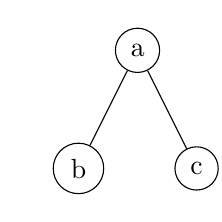
\begin{tikzpicture}

\node [circle,draw] (z){a}
  child {node [circle,draw] (a) {b}    
  }  
  child {node [circle,draw] (b) {c}
  };
\end{tikzpicture}
\caption{A 3 node binary tree.}

\end{center}
\end{figure}

Assume the probability of search for any of $a,b$, or $c$ is $\frac{1}{3}$. Under the three-way branch model, this can be done using exactly one comparison by asking if the key we are searching for is strictly less than $b$, equal to $b$, or strictly greater than $b$ and returning the correct key appropriately. Under a standard two-way branch model, this would require an extra comparison operation $\frac{2}{3}$ of the time as we can only distinguish one of the the three cases from the other two using a single two-way $<, >,$ or $=$ comparison operation. We get an expected cost of $1$ comparison in the three-way branch model and $\frac{5}{3}$ comparisons in the two-way model. In general, each comparison can reveal $3$ bits of information in the three-way model, while only $2$ bits per comparison can be revealed in the two-way model. 

\section{Why Study Binary Search Trees}

Binary search trees are ubiquitous throughout computer science with numerous applications. The basic binary search tree has extended in a number of ways. AVL trees (named after creators AdelsonVelskii and Landis) were the first form of self-balancing binary search trees introduced \cite{adelsonvelskii1963algorithm}. This type of tree was invented by the pair in 1963 and maintains a height of $O(\lg(n))$ (where $n$ is the number of nodes in the tree) during insertions and deletions (both of which take $O(\lg(n))$ time). Improved self-balancing binary search trees followed in the form of Symmetric binary B-trees by R. Bayer in 1972 \cite{bayer1972symmetric}. These are commonly referred to as red-black trees, a term coined by Guibas, Sedgewick and Robert in 1978 \cite{guibas1978dichromatic}. Allen and Munro followed with self-organizing binary search trees and examined a move to root heuristic, demonstrating its expected search time was within a constant of the optimal static binary tree \cite{allen1978self}. The famous splay trees of Sleator and Tarjan followed in 1985 \cite{sleator1985self}. Tango trees were invented in 2007 by Demaine et al. and provided the first $O(\lg \lg n)$-competitive binary tree \cite{demaine2007dynamic}. Here, $O(\lg \lg n)$-competitive means that the tango tree does at most $O(\lg \lg n)$ times more work (pointer movements and rotations) than an optimal offline tree. B trees are among the most commonly used binary tree variant and were invented in 1970 by R. Bayer and McCreight \cite{bayer1970organization}. \\

BST's and their extensions are integral to a large number of applications. For example, a BST variant known as the binary space partition is a method for recursviely subdividing space in order to store information in an easily accessible way. It is used extensively in 3D graphics \cite{schumacker1969study, paterson1992optimal}. Binary tries are similar to binary trees, but only store values for leaf nodes. Binary tries are routinely used in routers and IP lookup data structures \cite{song2010building}. Another example can be seen in the C++ \texttt{std::map} data structure, which is usually implemented using a red-black tree (another extension of binary search trees) in order to store its key-value pairs \cite{CppMap}. Finally, syntax trees (trees used in the parsing of various programming languages) are created using binary (and more complicated) tree structures. These trees are used in the parsing of written code during compilation \cite{louden1997compiler}.

\section{Overview}

In Chapter~\ref{Background and Related Work}, we review previous work done in the areas of binary search trees, multiway trees, alphabetic codes and various models of external memory. In Chapter~\ref{An Improved Bound for the Modified Minimum Entropy Heuristic}, we re-examine the modified entropy rule of G{\"u}ttler, Mehlhorn and Schneider \cite{guttler1980binary}. This is an $\Theta(n^2)$ time, $\Theta(n)$ space, algorithm for approximating the optimum binary search tree problem in the RAM model. The method works very well in practice, and the group had great experimental results, but unfortunately they could not bound the worst case expected cost as well as they would have hoped. While simpler solutions like the \textit{Min-max} and \textit{Weight Balanced} techniques of P. Bayer have worst case costs of at most $H+2$, the trio's modified entropy technique was only shown to have a worst case expected search cost of at most $c\cdot H+2$ where $c \approx 1.08$ \cite{bayer1975improved, guttler1980binary}. We provide a new argument of the modified entropy rule's worst case expected search cost and show that it is within an additive factor of entropy: at worst $H+4$. In Chapter~\ref{Approximate Binary Search in the Hierarchical Memory Model}, we move on to external memory models, examining the optimum binary search tree problem under the Hierarchical Memory Model of Aggarwal et al. \cite{aggarwal1987model}. We provide two algorithms which run in $O(n)$ time and bound their worst case expected costs. We show that the solutions provided both give a direct improvement over a solution of Thite provided under the related HMM$_2$ model \cite{thite2008optimum}. In Chapter~\ref{BST over Multisets}, we consider a variant of the optimum binary search tree problem (in the RAM model) where the set of probabilities given are from an unordered multiset. We show that for a multiset with $n$ probabilities, a simple greedy algorithm is within $\frac{n+1}{2n}$ of optimal. Finally, in Chapter~\ref{Conclusion and Open Problems}, we summarize our findings and discuss several problems which remain open.


\chapter{Background and Related Work} \label{Background and Related Work}

In this Chapter we provide an overview of relevant work on binary search trees, alphabetic codes, multiway search trees and models of external memory.

\section{Binary Search Trees}

In 1971, C. Gotlieb and Walker gave an approximate solution to the optimum binary search tree problem \cite{walker1971top}. Knuth shortly thereafter gave the first optimal solution \cite{knuth1971optimum}. Knuth's optimal solution requires $O(n^2)$ time and space which is too costly in many situations. Several others have since examined the approximate version of the problem. While unable to bound an approximate algorithm within a constant of the optimal solution, many authors have been able to bound the cost based on the entropy of the distribution of probabilities, $H$. Specifically, 
\begin{align*}
H = \sum_{i=1}^{n} p_i\cdot\lg(\frac{1}{p_i}) + \sum_{j=0}^{n} q_i\cdot\lg(\frac{1}{q_j}).
\end{align*}
In 1975, P. Bayer showed that 
\begin{align*}
H-\lg H-(\lg e-1) \leq C_{Opt} \leq C_{WB}, C_{MM} \leq H + 2
\end{align*}
where $C_{Opt}, C_{WB}$, and $C_{MM}$ are costs for the optimal solution, as well as weight-balanced and min-max heuristic methods respectively \cite{bayer1975improved}. Weight-balanced and min-max cost heuristics are greedy and require both $O(n)$ time and $O(n)$ space to run. These greedy heuristics use a top-down approach where the tree root is selected from among the $n$ keys, and we recurse in both the left and right subtrees. Let $P_L(B_i)$ and $P_R(B_i)$ represent the probabilities of searching for a key before or after key $B_i$ respectively. The Weight-balanced approach, makes this greedy root selection by picking the root $B_i$ such that $|P_L(B_i)-P_R(B_i)|$ is minimized.
  In 1980, G{\"u}ttler, Mehlhorn and Schneider presented a new heuristic, the modified entropy rule \cite{guttler1980binary} which built upon the ideas of Horibe \cite{horibe1977improved}. The Entropy Rule greedily selects $B_i$ as the root such that
\begin{align*}
H(P_L(B_i), p_i, P_R(B_i)) = P_L(B_i)\cdot\lg(\frac{1}{P_L(B_i)}) + p_i \cdot \lg(\frac{1}{p_i}) + P_R(B_i)\cdot\lg(\frac{1}{P_R(B_i)})  
\end{align*}
\noindent is maximized. As discussed in Chapter~\ref{An Improved Bound for the Modified Minimum Entropy Heuristic}, this was modified to improve its performance. G{\"u}ttler, Mehlhorn and Schneider gave empirical evidence that the heuristic out-performed others \cite{guttler1980binary}. While the heuristic took $O(n^2)$ time, it only required $O(n)$ space, a huge savings over the optimal solution. However, they were unable to prove that the cost of the modified entropy rule $C_{ME} \leq H+2$ (unlike previous weight-balanced and min-max heuristics) and settled with $C_{ME} \leq c_1\cdot H+2$ where $c_1=\frac{1}{H(\frac{1}{3}, \frac{2}{3})} \approx 1.08$. We re-examine this method and provide a new bound of $H+4$ in Chapter~\ref{An Improved Bound for the Modified Minimum Entropy Heuristic}. In 1993, De Prisco and De Santis presented a new heuristic for constructing a near-optimum binary search tree \cite{de1993binary}. The method is discussed in more detail in section~\ref{sec:deBST} and has an upper bounded cost of at most $H+1-q_0-q_n+q_{max}$ where $q_{max}$ is the maximum weight leaf node. This method was later updated by Bose and Dou\"{i}eb (and is also discussed in section~\ref{sec:deBST}) to have a worst case cost of \cite{bose2009efficient}
\begin{align*}
H + 1 - q_0 - q_n + q_{max} - \sum_{i=0}^{m'} pq_{\text{rank}[i]}.
\end{align*}
Here, $m'=\max({2n-3P,P})-1 \geq \frac{n}{2} - 1$ where $P$ is the number of increasing or decreasing sequences in a left-to-right read of the access probabilities of the leaves (gaps) and,  $pq_{\text{rank}[i]}$ is the $i^{th}$ smallest access probability among all keys and gaps except $q_0$ and $q_n$.

 
\section{Alphabetic Codes}

Determining the optimum alphabetic coding is an important related problem relevant later in this thesis. Given a set of $n$ keys (keys $B_1, ..., B_n$) with various probabilities, we wish to build a binary search tree where every internal node has two children, leaves have no children, and the $n$ keys described are the leaves. We wish to build the tree with the minimum expected search cost. The expected search cost is
\begin{align*}
\sum_{i=1}^{i=n} p_i \cdot d_T(B_i)
\end{align*}
where $p_i$ is the probability of searching for key $B_i$ and $d_T(B_i)$ is the depth of the leaf representing the key $B_i$ in the tree $T$. The alphabetic ordering of the leaves must be maintained. This is the same as the binary search tree problem with all internal node weights zero.

In 1952, Huffman developed the well known Huffman tree, which solved the same problem without a lexicographic ordering constraint on leaves \cite{huffman1952method}. Gilbert and Moore were the first to examine the problem with the added alphabetic constraint (alphabetical codes) and developed a $O(n^3)$ algorithm which solved the problem optimally \cite{gilbert1959variable}. Hu and Tucker gave a $O(n^2)$ time and $O(n)$ space algorithm in 1971 \cite{hu1971optimal} which was improved by Knuth to take only $O(n \lg n)$ time and $O(n)$ space in 1973 \cite{knuth1973sorting}. The original proof of Hu and Tucker was extremely complicated, but was later simplified by Hu \cite{hu1973new} and Hu et al. \cite{hu1979binary}. Garsia and Wachs gave an independent $O(n \lg n)$ time, $O(n)$ space algorithm in 1977 \cite{garsia1977new}. This new algorithm by Garsia and Wachs was shown to be equivalent to the Hu and Tucker algorithm in 1982 by Hu \cite{Hu1982Book} and also went through a proof simplification \cite{kingston1988new} by Kingston in 1988.

In 1991, Yeung proposed an approximate solution which solved the problem in $O(n)$ time and space \cite{yeung1991alphabetic}. The algorithm produced a tree with worst case cost $H + 2 - p_1-p_n$. This algorithm was later improved by De Prisco and De Santis who created an $O(n)$ time algorithm which has a worst case cost of $H+1-p_1-p_n+p_{max}$ \cite{de1993binary}. The method was improved one more time by Bose and Dou\"{i}eb who improved upon Yeung's method by decreasing the bound by $\sum_{i=0}^m p_{\text{rank}[i]}$ where $m=\max({n-3P,P})-1 \geq \frac{n}{4} - 1$, $P$ is the number of increasing or decreasing sequences in a left-to-right read of the access probabilities of the leaves and $p_{\text{rank}[i]}$ is the $i^{th}$ smallest access probability among all leaves except $p_1$ and $p_n$ \cite{bose2009efficient}. Replacing Yeung's method with the improved algorithm of Bose and Dou\"{i}eb in the De Prisco and De Santis algorithm gave the tightest bound seen so far of 
\begin{align*}
H+1+\sum_{i=1}^{n}p_i-p_1-p_n-\sum_{i=0}^m p_{\text{rank}[i]}. 
\end{align*}

\section{Multiway Trees} \label{sec:MWT}


Another related problem is the static k-ary or multiway search tree problem. It is similar to optimum binary search tree problem with the added option that up to $k-1$ keys can be placed into a single node, and the cost of search within a node is constant. Multiway search trees maintain an ordering property similar to that of traditional binary search trees. Each key in every page $g$ that isn't the root page must have its keys lie between some keys $l$ and $l'$, two keys located in $g's$ parent. Each internal node of the k-ary tree contains at least one and at most $k-1$ keys while a leaf node contains no keys and represents searching for an item in a gap between keys. Successful searches end in an internal node while unsuccessful searches end in one of the $n+1$ leaves of the tree. The cost of search is the average path depth which is defined as:

\begin{align*}
\sum_{i=1}^{n} p_i(d_T(B_i)+1) + \sum_{j=0}^{n} q_j(d_T((B_{i-1},B_i)))
\end{align*}

\noindent where $B_i$'s represent successful search keys with probabilities $p_i$, pairs $(B_{i-1},B_i)$ (with probabilities $q_{i-1}$) represent gaps and $d_T(B_i)$  or $d_T((B_{i-1},B_i))$ represent the depth of keys or gaps respectively in the tree $T$.

Vishnavi et al. \cite{vaishnavi1980optimum}, and Gotlieb  \cite{gotlieb1981optimal} in 1980 and 1981 respectively independently solved the problem optimally in $O(k\cdot n^3)$ time. In a slightly modified B-tree model (every leaf has the same depth, every internal node is at least half full), Becker's 1994 work gave a $O(kn^{\alpha})$ time algorithm where $\alpha=2+log2/log(k+1)$ \cite{becker1994new}. Later, in 1997, Becker propsed an $O(Dkn)$ time algorithm where D is the height of the resulting tree \cite{becker1997construction}. The algorithm did not produce an optimal tree but was thought to be empirically close despite having no strong upper bound. In 2009, Bose and Dou\"{i}eb gave both an upper and lower bound on the optimal search tree in terms of the entropy of the probability distribution as well as an $O(n)$ time algorithm to build a near-optimal tree \cite{bose2009efficient}. Their bounds of
\begin{align*}
\frac{H}{\lg(2k-1)} \leq P_{OPT} \leq P_T \leq \frac{H}{\lg k} + 1 + \sum_{i=0}^n q_i - q_0 - q_n - \sum_{i=0}^m q_{\text{rank}[i]}
\end{align*}
is discussed in more detail in section~\ref{43} of this paper. Here, $m=max({n-3P,P})-1 \geq \frac{n}{4} - 1$. $P$ is the number of increasing or decreasing sequences in a left-to-right read of the access probabilities of the gaps. Moreover, $q_{\text{rank}[i]}$ is the $i^{th}$ smallest access probability among all leaves (gaps) except $q_0$ and $q_n$.

\section{Memory Models}

In the typical RAM model, we assume that all reads and writes from memory take a constant amount of time. While this is a valid assumption in many situations (both in the context of theory and programming) when dealing with very large data sets, this is simply not the case. A typical computer has a memory hierarchy with CPU registers, various levels of cache, RAM, SSD and/or hard drives. Each of these memory levels has increasing size but decreasing I/O speed. Typically, the difference between the levels is dramatic (reading from disk takes roughly a million times longer than accessing a CPU register) \cite{vitter2001external}. Moreover, many memory hierarchies allow blocks of memory to be moved quickly after a single key or cache line has been accessed. It is thus possible to take advantage of the locality of data during computations. Moreover, it is imperative to consider memory I/O speeds, especially when the dataset being worked on does not fit on internal memory. \textit{External memory} algorithms and data structures refer to those methods and structures which explicitly manage data placement and movement \cite{vitter2001external}. Various authors have created models to properly reflect the performance of such algorithms and data structures, and we consider the optimum binary search tree problem under such a model.

In Chapter~\ref{Approximate Binary Search in the Hierarchical Memory Model}, we discuss the optimum binary search tree problem under the 1987 Hierarchical Memory Model of Aggarwal et al. \cite{aggarwal1987model}. The model is described thoroughly in section~\ref{The Hierarchical Memory Model}, but essentially provides an alternative to the classic RAM model. It simulates a memory hierarchy with various memory sizes and different access times for each type of memory. The model does have its shortcomings though as it does not provide us with the ability to move blocks of memory between these different memory types (as in a typical computer). The HMM model was later extended to the Hierarchical Memory with Block Transfer Model of Aggarwal, Chandra, and Snir \cite{aggarwal1987hierarchical}. This model provides a less artificial setting by allowing for contiguous blocks of memory to be copied from one location to another for a cheaper price. The cost of this copy equal to the cost to access the most expensive location being copied (to or from), plus the size of the block.


As explained in the survey of Vitter, several other models of external memory have followed \cite{vitter2001external}. Work has been done to consider models with parallelism. Vitter and Shriver built upon the HMM and HMBTM models of Aggarwal et al. \cite{aggarwal1987model, aggarwal1987hierarchical} in order to allow parallelism \cite{vitter1994algorithms}. This updated model connects $P$ parallel memory hierarchies at their base memory levels. In 1994, Alpern et al. introduced the Uniform Memory Hierarchy (UMH) \cite{alpern1994uniform}. The UMH considers block sizes and bandwidths between memory levels, and allows for simultaneous transfer between pairs of memory levels. The UMH was considered with additional parallelization by Vitter and Nodine \cite{vitter1993large}.


Cache-oblivious algorithms were introduced by Frigo, Leiserson, Prokop and Ramachandran in 1999 \cite{frigo1999cache}. The model used is the ideal-cache model which has a two-level memory hierarchy. The internal memory (named cache) has $Z$ words and the main memory is arbitrarily large. The cache is divided into cache lines of size $L$ and it is assumed that $Z=\Omega(L^2)$ (the tall cache assumption). Frigo et. al examined the fast fourier transform and matrix multiplication under this model. Many others have since used this model and examined problems in a cache-oblivious setting such as the cache-oblivious b-trees of Bender et. al \cite{bender2000cache}, the funnel heap of Brodal et. al \cite{brodai2002funnel}, or the locality preserving cache-oblivious dynamic dictionary of Bender et. al \cite{bender2002locality}.

A complete and thorough explanation of memory hierarchies (especially those considered before cache-oblivious settings) can be found in the survey of Vitter \cite{vitter2001external}.



\chapter{An Improved Bound for the Modified Minimum Entropy Heuristic}\label{An Improved Bound for the Modified Minimum Entropy Heuristic}

In this chapter we show that the Modified Minimum Entropy Heuristic of G{\"u}ttler, Mehlhorn and Schneider \cite{guttler1980binary} is within an additive factor of entropy: at worst $H+4$.

\section{Preliminaries}

Recall \ref{1.1}, $H = \sum_{i=1}^{n} p_i\cdot\lg(\frac{1}{p_i}) + \sum_{j=0}^{n} q_i\cdot\lg(\frac{1}{q_j})$. We also use
\begin{align*}
H(x_1,x_2,...,x_n) = \sum_{i=1}^{n} x_i\cdot\lg(\frac{1}{x_i})
\end{align*} to describe the entropy of any probability distribution $(x_1, x_2, ...., x_n)$. For subtree $t$, we let 
\begin{align*}
p_t=\sum_{i : B_i \in t} p_i + \sum_{i : (B_i, B_{i+1}) \in t} q_i
\end{align*}
 be its total probability (the sum of the probability of all nodes within the subtree). $P_{L}(B_i)$ and $P_{R}(B_i)$ are probabilities of searching lexicographically before or after (respectively) key $B_i$. $P_{L}(B_i, B_{i+1})$ and $P_{R}(B_i, B_{i+1})$ are probabilities of searching lexicographically before (or equal to) $B_i$ and after (or equal to) $B_{i+1}$ respectively. For a subtree $t$, $P_{L_t}(B_i)$ and $P_{R_t}(B_i)$ describe the normalized probabilities of searching for a key to the left or right of $B_i$ within $t$, and $P_{L_t}(B_i,B_{i+1})$ and $P_{R_t}(B_i,B_{i+1})$ have analogous definitions. 
We let  
\begin{equation}
E_t=H(P_{L_t}(B_i), \frac{p_i}{p_t}, P_{R_t}(B_i))
\end{equation} be the local entropy of a subtree $t$ rooted at key $B_i$.  

\section{The Modified Entropy Rule}\label{The Modified Entropy Rule}

We first describe the entropy rule for greedy root selection then explain how it was modified in \cite{guttler1980binary}. For a subtree $t$ with probability $p_t$, the entropy rule greedily chooses the key $B_i$ as the root such that $H(P_{L_t}(B_i), \frac{p_i}{p_t}, P_{R_t}(B_i))$ is maximized. While this rule behaves quite well in practice, certain cases cause it to have poor performance (refer to Figure 3.1). 


\begin{figure}[H]
\centering
% Set the overall layout of the tree
\tikzstyle{level 1}=[level distance=3cm, sibling distance=3cm]
\tikzstyle{level 2}=[level distance=3cm, sibling distance=3cm]
\scriptsize
\begin{subfigure}{.46\textwidth}
\centering
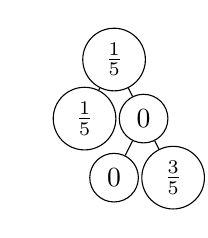
\begin{tikzpicture}[scale=0.5]
\node [circle,draw] (z){$\frac{1}{5}$}
  child {node [circle,draw] (a) {$\frac{1}{5}$}    
  }  
  child {node [circle,draw] (b) {$0$}
	  child {node [circle,draw] (e) {$0$}}
	  child {node [circle,draw] (f) {$\frac{3}{5}$}}
  };
\end{tikzpicture}
\caption{Entropy rule tree: $C=\frac{8}{5}$}
\end{subfigure}
\begin{subfigure}{.46\textwidth}
\centering
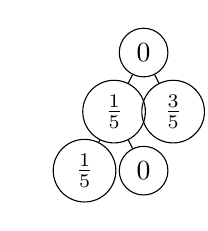
\begin{tikzpicture}[scale=0.5]
\node [circle,draw] (z){$0$}
  child {node [circle,draw] (a) {$\frac{1}{5}$} 
  	child {node [circle,draw] (e) {$\frac{1}{5}$}}
	  child {node [circle,draw] (f) {$0$}}   
  }  
  child {node [circle,draw] (b) {$\frac{3}{5}$}
  };
\end{tikzpicture}
\caption{Modified entropy rule tree: $C=\frac{7}{5}$}
\end{subfigure}
\caption{Comparison of entropy and modified entropy rule heuristics}
\end{figure}

Figure 3.1 demonstrates the shortcomings of the entropy rule heuristic. Given the probability set $\{q_0 = \frac{1}{5}, p_1 = \frac{1}{5}, q_1 = 0, p_2 = 0, q_3 = \frac{3}{5}\}$ the entropy rule will mistakenly choose key $B_1$ as the root while selecting $B_2$ as the root produces a better tree. This mistake is remedied in the modified entropy rule of G{\"u}ttler, Mehlhorn and Schneider \cite{guttler1980binary}. The modified entropy heuristic chooses the root in of the following three ways:

\begin{enumerate}[label=\alph*)]
\item If there exists key $B_i$ such that $\frac{p_i}{p_t} > \max(P_{L_t}(B_i), P_{R_t}(B_i))$ we always select $B_i$ as the root.

\item If there exists a gap $(B_i, B_{i+1})$ such that $\frac{q_i}{p_t} > max(P_{L_t}(B_i, B_{i+1}), P_{R_t}(B_i, B_{i+1}))$ then we select the root from among $B_i$ and $B_{i+1}$. $B_i$ is chosen if $P_{L_t}(B_i, B_{i+1}) > P_{R_t}(B_i, B_{i+1})$ and $B_{i+1}$ is chosen otherwise.

\item Otherwise, $B_i$ is selected such that $H(P_{L_t}(B_i), \frac{p_i}{p_t}, P_{R_t}(B_i))$ is maximized (as in the original entropy rule).

\end{enumerate}

The approach proposed by G{\"u}ttler, Mehlhorn and Schneider takes $O(n^2)$ time in the worst case and $O(n)$ space.

\section{Modified Entropy is Within 4 of Entropy}

First, we review a quick Lemma about entropy (nearly identical to Lemma 2.3 in \cite{bayer1975improved}).

\begin{lem}\label{entr2x}
If $x \leq \frac{1}{2}$ then $H(x, 1-x) \geq 2x$.
\end{lem}
\begin{proof}
We refer the reader to Gallager's 1968 work \cite{gallager1968information}.
\end{proof}

Next, we describe a Lemma which breaks our choice of root in the greedy modified entropy heuristic into one of three cases (not to be confused with the three \textit{rules} used in~\ref{The Modified Entropy Rule}). 

\begin{lem}\label{MECases}
When using the modified entropy rule chooses the root $B_r$ of a subtree $t$ with total probability $p_t$, one of the following three cases must occur: 
\begin{align*}
&\text{Case 1) } E_t \geq 1-2 \frac{p_r}{p_t} \\
&\text{Case 2) There exists gap}  (B_i, B_{i+1}) \text{ such that } \frac{q_i}{p_t} > max(P_{L_t}(B_i, B_{i+1}), P_{R_t}(B_i, B_{i+1}))\\
&\text{Case 3) }  \max(P_{L_t}(B_r), P_{R_t}(B_r)) < \frac{4}{5}
\end{align*}

\end{lem}
\begin{proof} At a high level, we first show that \textit{Rule a} from~\ref{The Modified Entropy Rule} implies \textit{Case 1}. We also show that if there exists $p_i$ such that $\frac{p_i}{p_t} > \max(P_{L_t}(B_i), P_{R_t}(B_i))$, but cannot apply \textit{Rule a}, then we still have \textit{Case 1}. Assuming that neither of the two aforementioned conditions occur, we must have that there exists some gap $(B_i, B_{i+1})$ spanning the middle of the data set. Given this condition, we show that if \textit{Case 2} does not occur (i.e. we cannot use \textit{Rule b}~\ref{The Modified Entropy Rule}) then \textit{Case 3} must occur, completing the proof. 


\noindent\textbf{\textit{Rule a) $\implies$ Case 1}} \\
 First, suppose there exists some $p_i$ such that $\frac{p_i}{p_t} > \max(P_{L_t}(B_i), P_{R_t}(B_i))$. By the \textit{Rule c)}~\ref{The Modified Entropy Rule}, it must be selected as the root and thus $r=i$. Moreover, both $P_{L_t}(B_i)$ and $P_{R_t}(B_i))$ must be less than one half. Thus, using \ref{entr2x} we have: 
\begin{align*}
E_t &\geq H( max(P_{L_t}(p_i), P_{R_t}(p_i)), 1-max(P_{L_t}(p_i), P_{R_t}(p_i)) \\
 &\geq 2\cdot \max(P_{L_t}(p_i), P_{R_t}(p_i)) \\  &\geq 1-\frac{p_i}{p_t} \\ 
 &\geq 1-2 \frac{p_i}{p_t} = 1-2 \frac{p_r}{p_t} 
\end{align*}
 as required. \\
 
\noindent\textbf{\textit{$B_i$ spans middle $\implies$ Case 1}} \\
If we do not have some $p_i$ such that $\frac{p_i}{p_t} > \max(P_{L_t}(B_i), P_{R_t}(B_i))$ but do have some $B_i$ such that $P_{L_t}(B_i) \leq \frac{1}{2}$ and $P_{R_t}(B_i) \leq \frac{1}{2}$) then we must use \textit{Rule c}~\ref{The Modified Entropy Rule}. We then must have that:
\begin{align*}
 E_t &\geq H(P_{L_t}(B_i), \frac{B_i}{p_t} , P_{R_t}(B_i)) \text{ and} \\
 0 &\leq P_{L_t}(B_i) \leq 0.5 \text{ and}\\
 0 &\leq \frac{p_i}{p_t} \leq 0.5 \text{ and}\\
 0 &\leq P_{R_t}(B_i) \leq 0.5
\end{align*} 
   then we know that \\
\begin{align*}
H(P_{L_t}(p_i), \frac{p_i}{p_t} , P_{R_t}(p_i)) \geq H(1/2, 1/2) = 1
\end{align*}
in this case.
 Thus, combining the above two cases, if have some $B_i$ such that $P_{L_t}(B_i) \leq \frac{1}{2}$ and $P_{R_t}(B_i) \leq \frac{1}{2}$ then $E_t \geq 1-2p_r$ as required. \\

\noindent\textbf{\textit{$\big($NOT($B_i$ spans mid) AND NOT(Case 1) AND NOT(Case 2)$\big)$ $\implies$ Case 3}} \\
Otherwise, we must have some gap $(B_i, B_{i+1})$ spanning the middle of the data set (i.e. $P_{L_t}(B_i, B_{i+1}) < \frac{1}{2}$ and $P_{R_t}(B_i, B_{i+1}) < \frac{1}{2}$). Suppose that \textit{Case 2} does not occur (i.e. we cannot use \textit{Rule b}): there does not exist a $(B_i, B_{i+1})$ such that $\frac{q_i}{p_t} > max(P_{L_t}(B_i, B_{i+1}), P_{R_t}(B_i, B_{i+1}))$. Then, for any root $r$ of $t$ we have that \\
\begin{align*}
\max(P_{L_t}(B_r), P_{R_t}(B_r)) &\geq \min(P_{L_t}(B_r), P_{R_t}(B_r))\\ 
\max(P_{L_t}(B_r), P_{R_t}(B_r)) &\geq q_i
\end{align*}
Thus, for any root $r$:
\begin{align*}
\max(P_{L_t}(p_r), P_{R_t}(p_r)) \geq 1/3
\end{align*}
 and by our assumption 
\begin{align*}
\max(P_{L_t}(p_r), P_{R_t}(p_r)) < \frac{1}{2}.
\end{align*}
 So, as in the proof of table 3 (5.3) in \cite{guttler1980binary}\\
\begin{align*}
E_t \geq H(1/3, 2/3) \approx 0.92.
\end{align*}
Either \textit{Case 1} occurs, or we have that:
\begin{align*}
E_t &< 1-2\frac{p_r}{p_t} \\
\implies \frac{p_r}{p_t} &< \frac{1-H(\frac{1}{3}, \frac{2}{3})}{2} \approx 0.04.
\end{align*}

Suppose for contradiction that $\max(P_{L_t}(p_r), P_{R_t}(p_r)) \geq \frac{4}{5} p_t$ then we have:
\begin{align*}
E_t \leq H(\frac{4}{5}, \frac{1-H(\frac{1}{3}, \frac{2}{3})}{2}, \frac{1}{5}-\frac{1-H(\frac{1}{3}, \frac{2}{3})}{2}) \approx 0.87 < 0.92 \approx H(\frac{1}{3}, \frac{2}{3}) \leq E_t
\end{align*}
which is a contradiction.
Thus, if we do not have \textit{Case 1} or \textit{Case 2} we must have \textit{Case 3} which completes the proof.



\end{proof}

Before we examine the main theorem we show a small claim.

\newtheorem{claim}{Claim}
\begin{claim}\label{Claim1}
$H(\frac{1}{2}-\frac{1}{2} x, \frac{1}{2} + \frac{1}{2} x) \geq 1- \frac{4}{5} x^2$ when $0 < x < \frac{1}{2}$
\end{claim}

\begin{proof}
In order to prove the claim, we find the minimum of
\begin{align*}
H(\frac{1}{2}-\frac{1}{2} x, \frac{1}{2} + \frac{1}{2} x) - (1 - \frac{4}{5} x^2) 
\end{align*}
when $0 < x < \frac{1}{2}$. To do this, we define $F(x)$ and take the derivative with respect to $x$.
\begin{align*}
F(x) &= H(\frac{1}{2}-\frac{1}{2} x, \frac{1}{2} + \frac{1}{2} x) - (1 - \frac{4}{5} (x)^2) \\
F(x) &= - (\frac{1}{2}-\frac{1}{2} x)\cdot \lg(\frac{1}{2}-\frac{1}{2} x) - (\frac{1}{2} + \frac{1}{2} x)\cdot\lg(\frac{1}{2} + \frac{1}{2} x) - (1 - \frac{4}{5} x^2) \\
\implies F'(x) &= \lg(\frac{1}{2}-\frac{1}{2} x) - \lg(\frac{1}{2} + \frac{1}{2} x) + \frac{8}{5}x \text{ (with some careful manipulation)}
\end{align*}

The only root occurs when $x = 0$. Thus, we check when $x \rightarrow 0$ and $x \rightarrow \frac{1}{2}$. We note that: \\
\begin{align*}
&F'(x) \xrightarrow{x \to 0} 0^{+}  \text{ and} \\
&F'(x) \xrightarrow{x \to \frac{1}{2}} 0.0112781 > 0
\end{align*}
Thus, $H(\frac{1}{2}-\frac{1}{2} x, \frac{1}{2} + \frac{1}{2} x) - (1 - \frac{4}{5} (x)^2) > 0$ for $ 0 < x < \frac{1}{2}$ which proves the claim.
\end{proof} 


\begin{thm}
Let $C_{ME}$ be the expected cost of search for a tree made by the modified entropy rule.
\begin{align*}
C_{ME} \leq H + 4
\end{align*}
\end{thm}

\begin{proof}
This uses a similar style to the proof of theorem 4.4 in \cite{bayer1975improved}.
We bind each $E_t$ for each subtree of our BST on a case by case basis using the cases of Lemma~\ref{MECases}.\\
If \textit{Case 1} occurs, we obviously have that
\begin{equation}\label{EQC1}
E_t \geq 1-2 \frac{p_r}{p_t}
\end{equation}
Note that this can only happen once for each key (a key can only be root once). \\

As mentioned in Lemma~\ref{MECases} if some $B_i$ spans in the middle of the data set, $P_{L_t}(B_i) \leq \frac{1}{2}$ and $P_{R_t}(B_i) \leq \frac{1}{2}$, we can still show that \textit{Case 1} occurs. Suppose for the remainder of the proof that there is no such middle-spanning $B_i$.

Let $(B_m, B_{m+1})$ be the unique middle gap (i.e. $P_{L_t}(B_m, B_{m+1}) < \frac{1}{2}$ and $P_{R_t}(B_m, B_{m+1}) < \frac{1}{2}$) when \textit{Case 2} or \textit{Case 3} occurs. When \textit{Case 2} occurs, we know that we could select a root from among the two keys outside of our middle spanning gap, and choose the one which is closer to the middle. Thus, we have that (using Lemma~\ref{entr2x}):
\begin{equation}\label{EQC2} 
E_t \geq H(\frac{1}{2}-\frac{1}{2} \frac{q_m}{p_t}, \frac{1}{2} + \frac{1}{2} \frac{q_m}{p_t}) \geq 2(\frac{1}{2}-\frac{1}{2} \frac{q_m}{p_t})=1-\frac{q_m}{p_t}.
\end{equation}
Note that by the definition of the \textit{Rule c}~\ref{The Modified Entropy Rule}, when this occurs, $(B_m, B_{m+1})$ must be a leaf of depth at most 2. Thus, this condition can only happen twice for each $(B_m, B_{m+1})$ gap. \\

When neither \textit{Case 1} nor \textit{Case 2} occur (and we have a $(B_m, B_{m+1})$ spanning the middle) we must have \textit{Case 3}. This gives us:
\begin{align*}
E_t \geq H(\frac{1}{2}-\frac{1}{2} \frac{q_m}{p_t}, \frac{1}{2} + \frac{1}{2} \frac{q_m}{p_t})
\end{align*}
We again apply Claim~\ref{Claim1} and get:
\begin{equation}\label{EQC3}
E_t \geq 1- \frac{4}{5} (\frac{q_m}{p_t})^2
\end{equation}

As in \cite{bayer1975improved} we define a $b_t$ for each subtree $t$ as follows. We want to have a value for $b_t$ such that $E_t \geq 1 - \frac{b_t}{p_t}$ in all cases. Using \textit{Cases 1,2}, and \textit{3} are their respective equations~\ref{EQC1},~\ref{EQC2}, and~\ref{EQC3} we do just that: \\
Let $b_t=2\cdot p_r$ when \textit{Case 1} occurs. $B_r$ is the root of $b_t$. \\
Let $b_t=2\cdot q_m$ when \textit{Case 2} occurs. $(B_m, B_{m+1})$ is middle gap of $b_t$. \\
Let $b_t=\frac{q_m^2}{p_t}$ when \textit{Case 3} occurs. $(B_m, B_{m+1})$ is middle gap of $b_t$. \\


Note that, in 1975 P. Bayer showed that the cost $C$ of our tree could be defined as (\textbf{Lemma 2.3} \cite{bayer1975improved}): \\
\begin{align*}
C = \sum_{t \in S_T} p_t
\end{align*}
and the entropy could be calculated by
\begin{align*}
H = \sum_{t \in S_T} p_t \cdot E_t
\end{align*}  
where $S_T$ is the set of all subtrees of our tree $T$. \\

\noindent Thus, by subbing in $E_t \geq 1 - b_t$ and rearranging we get: 
\begin{align*}
&H = \sum_{t \in S_T} p_t \cdot E_t \geq \sum_{t \in S_T} p_t - \sum_{t \in S_T} b_t = C - \sum_{t \in S_T} b_t \\
 \implies &C \leq H + \sum_{t \in S_T} b_t
\end{align*}
As mentioned above, \textit{Case 1} and \textit{Case 2} can only occur once and twice respectively for any potential root $B_r$ or gap $(B_m, B_{m+1})$. \textit{Case 3} however, can occur many times for a gap $(B_m, B_{m+1})$. Each time it occurs though, $\frac{q_m}{p_t}$ must increase by a factor of at least $\frac{5}{4}$ since $\max(P_{L_t}(B_r), P_{R_t}(p_r)) < \frac{4}{5}$ for the root $B_r$ of the subtree by \textit{Case 3)} of Lemma~\ref{MECases}. Moreover, if $\frac{q_m}{p_t} > \frac{1}{2}$ then we will have \textit{Case 2}. Let $S_m$ be the set of all subtrees $t$ for which $(B_m, B_{m+1})$ is the middle gap and \textit{Case 3} only applies. We have that
\begin{align*}
C \leq H + \sum_{t \in S_T} b_t = H + 2 \sum\limits_{r = 1}^n p_r + 2 \sum\limits_{m = 0}^n q_m + \sum\limits_{m = 0}^n \sum\limits_{t \in S_m} \frac{4}{5}\frac{q_m^2}{p_t}
\end{align*}
 \\ 
By factoring out $q_m$ and examining only cases up to $\frac{q_m}{p_t} = \frac{1}{2}$ (since otherwise \textit{Case 2} will occur) we get:
\begin{align*}
C &\leq H + 2 + \sum\limits_{m = 0}^n (\frac{4}{5} \cdot q_m) \sum\limits_{x=0}^{\infty} \frac{1}{2} \cdot (\frac{4}{5}) ^ x \\
C &\leq H + 2 + \sum\limits_{m = 0}^n \frac{4}{5} \cdot q_m \cdot \frac{1}{2} \cdot (\frac{1}{1-\frac{4}{5}}) \text{    (geometric series)} \\
C &\leq H + 2 + 2\cdot \sum\limits_{m = 0}^n q_m \\
C &\leq H + 4
\end{align*}

\end{proof}

It remains open as to whether or not this bound is tight. We conjecture that it is likely the case that the worst case bound is in fact $H+2$ as no cases with worse behaviour are known.

\chapter{Approximate Binary Search in the Hierarchical Memory Model}\label{Approximate Binary Search in the Hierarchical Memory Model}
 
In this chapter we examine the optimum BST problem under the Hierarchical Memory Model (HMM) model. We provide two approximate solutions, bound their worst case expected costs via entropy, and show improvement over a previous solution in the related HMM$_2$ model. 
 
\section{The Hierarchical Memory Model}\label{The Hierarchical Memory Model}

The HMM was proposed in 1987 by Aggarwal et al. as an alternative to the classic RAM model \cite{aggarwal1987model}. It was intended to better model the multiple levels of the memory hierarchy. The model has an unlimited number of registers, $R_1, R_2, ...$ each with its own location in memory (a positive integer). In the first version of the model, accessing a register at memory location $x_i$ takes $\lceil \lg(x_i) \rceil$ time. Thus, computing $f(a_1, a_2, ..., a_n)$ takes $\sum_{i=1}^{n} \lceil \lg(location(a_i)) \rceil$ time. The original paper also considered arbitrary cost functions $f(x)$. We will use the cost function as was explained in Thite's thesis \cite{thite2008optimum}. Here, $\mu (a)$ is the cost of accessing memory location $a$. We have a set of memory sizes $m_1, m_2, ..., m_l$ which are monotonically increasing. Each memory level has a finite size except $m_l$ which we assume has infinite size. Each memory level has an associated cost of access $c_1, c_2, ..., c_l$. We assume that $c_1 < c_2 < ... < c_l$. The cost of accessing a memory location $a$ is given by
\begin{equation}
\mu (a) = c_i \text{ if } \sum_{j = 1}^{i-1}m_j  < a \leq \sum_{j = 1}^{i}m_j.
\end{equation}

\noindent More specifically, we can think of $c_i$ as the entire cost of moving a element in $m_i$ recursively up the memory hierarchy and finally accessing it. While there is interesting problems in more sophisticated models, it is beyond the scope of this work to examine locality optimizations under a more complex model in this recursive movement of items up the hierarchy.

Thite notes that typical memory hierarchies have decreasing sizes for faster memory levels (moving \textit{up} the memory hierarchy). We make the same assumption:
\begin{align*}
m_1 < m_2 < ... < m_l.
\end{align*}
Unlike Thite, we also explicitly assume that successive memory level sizes divide one another evenly:
\begin{align*}
\forall i \in  \{1,2,...,l-1\} m_i \mid m_{i+1}.
\end{align*}

\section{Thite's Optimum Binary Search Trees on the HMM Model}

Thite's thesis provides solutions to several problems in the HMM and the related HMM$_2$ models \cite{thite2008optimum}. He first provides an optimal solution to the following problem (known as \textbf{Problem 5} in the work). Note that we have made slight modifications in order to maintain correct notation throughout this work:

\begin{quote}
\noindent \textit{\textbf{Problem 1 [Optimum BST Under HMM].} Suppose we are given a set of $n$ ordered keys $B_1, B_2, ..., B_n$ with associated probabilities of search $p_1, p_2, ..., p_n$, as well as $n+1$ ranges or gaps $(B_0, B_1), (B_1, B_2), ..., (B_{n-1}, B_n), (B_n, B_{n+1})$ with associated probabilities of search $q_0, q_1, ..., q_n$. The problem is to construct a binary search tree $T$ over the set of keys and gaps (keys must be internal nodes, and gaps must be leaves) and compute a memory assignment function $\phi : V (T) \rightarrow {1, 2, ..., n}$ that assigns nodes of $T$ to memory locations such that the expected cost of a search is minimized under the HMM model} \cite{thite2008optimum}.
\end{quote}

\noindent Note that we assume that $B_0$ represents $- \infty$ and $B_{n+1}$ represents $\infty$.

Thite provided three separate optimum solutions to the problem described; \textbf{Parts}, \textbf{Trunks}, and \textbf{Split}. Here, $h$ is the minimum memory level such that all $n$ keys can fit on memories of height at most $h$. More specifically $h$ is defined as \\
\begin{align*}
\min(h \in \{1,..,l\} ): n \leq \sum_{i = 1}^{h}m_i
\end{align*}

\noindent We now give a high-level overview the the three solutions of Thite. For a more detailed explanation, please refer to his thesis \cite{thite2008optimum}.

\textbf{Parts} is a bottom up dynamic programming algorithm which constructs optimum subtrees $T^{*}_{i,j}$ for each $i,j$, $1 \leq i \leq j \leq n$ using only the first $j-i+1$ memory locations. For each choice of root $B(k)$ where $k \in \{i, ..., j\}$ all possible memory assignments are examined. Thite claims a running time of $O(\frac{2^{h-1}}{(h-1)!}\cdot n^{2h+1})$ for the algorithm.

\textbf{Trunks} is an algorithm that, like parts, using dynamic programming to build optimal subtrees over larger and larger sets of keys. For each range $i,j$, $1 \leq i \leq j \leq n$, and for each possible root $B(k)$, they examine all $s$ such that $s \leq j-i+1$ and consider placing $s$ nodes in the first $h-1$ levels of memory, and the remaining $j-i-1-s$ nodes in memory level $h$. Thite claims that the algorithm takes $O(\frac{2^{n-m_h}\cdot (n-m_h+h)^{n-m_h}\cdot n^3}{(h-2)!})$ time. Moreover, the algorithm should work well in practice when $n-m_h$ and $h$ are small (i.e. a short memory hierarchy with a very large biggest memory size, typical in a modern computer).

\textbf{Split} is a top-down algorithm for solving the problem when there are $n$ levels in the memory hierarchy. Thite claims a running time of $O(2^n)$. We note that this running time result is dubious as Thite's explanation simply states that a root is chosen by examining each of the $2^{n-1}$ ways of partitioning memory locations between the left and right subtrees and recursing on each side. It is unclear how the potential roots are compared, and we cannot think of a way to select the correct root in this fashion without an exponential running time. A proof of correctness of algorithm was unfortunately omitted from Thite's work.

 In the following sections, we provide two approximate solutions to this problem that run in time $O(n)$ and provide an upper bound on their expected search costs. 
 
Thite also considered the same problem under the related HMM$_2$ model. This model assumes there are simply two levels of memory of size $m_1$ and $m_2$ with costs of access $c_1$ and $c_2$ where $c_1 < c_2$. Thite provides an optimal solution to this problem (named \textbf{TwoLevel}) he claims runs in time $O(n^5)$.
TwoLevel has two phases and in the first phase, it uses an algorithm similar to that of Knuth, solving for all subtrees that will fit on a single memory level (i.e. solves for all ranges $[i,j]$ such that $j-i+1 \leq \max(m_1, m_2))$. Specifically, it creates arrays $C[i,j]$ and $R[i,j]$ where C and R are the optimal tree cost (using a uniform cost model), and root selection of optimal tree over $[i,j]$.
TwoLevel phase two utilizes algorithm parts and uses dynamic programming to compute $c(i,j,n_1,n_2)$ and $r(i,j,n_1, n_2)$ which are the optimal tree and optimal tree root choices using the HMM$_2$ cost model using keys $[i,j]$ with $n_1$ keys in memory $M_1$ and $n_2$ in memory $M_2$. $c$ and $r$ are computed using dynamic programming. Thite claims the algorithm runs in $o(n^5)$, if $m_1 \in o(n)$, and in $O(n^4)$ if $m_1 \in O(1)$. He also gives an $O(n\lg n)$ time approximate solution with an upper bounded expected search cost of $c_2(H+1)$. This algorithm utilizes a $O(n)$ BST approximation algorithm of Mehlhorn \cite{mehlhorn1984sorting} and an $O(n \lg n)$ greedy scheme for placing the BST tree into memory. The solution we provide under the HMM model also gives an improvement over Thite's approximate algorithm in both running time and expected cost under the HMM$_2$ model.


\section{Efficient Near-Optimal Multiway Trees of Bose and Dou\"{i}eb}\label{43}

In order to obtain a good approximate solution to the optimum BST problem under the HMM model, we use the multiway search tree construction algorithm of Bose and Dou\"{i}eb. In 2009, they devised a new method with linear running time (independent of the size of a node in tree) and with the best expected cost to date \cite{bose2009efficient}. The group was able to prove that:
\begin{align*}
\frac{H}{\lg(2k-1)} \leq P_{OPT} \leq P_T \leq \frac{H}{\lg k} + 1 + \sum_{i=0}^n q_i - q_0 - q_n - \sum_{i=0}^m q_{\text{rank}[i]}.
\end{align*}

Here, H is the entropy of the probability distribution, $P_{OPT}$ is the average path-length (expected cost of search) in the optimal tree, $P_T$ is the average path length of the tree built using their algorithm and $m=max({n-3P,P})-1 \geq \frac{n}{4} - 1$. $P$ is the number of increasing or decreasing sequences in a left-to-right read of the access probabilities of the gaps. Moreover, $q_{\text{rank}[i]}$ is the $i^{th}$ smallest access probability among all leaves (gaps) except $q_0$ and $q_n$. Finally, $k$ is the size of a node in the tree (the number of keys that fit inside an internal node). Each node will have at most $k+1$ children. \\

As described in the section~\ref{sec:MWT}, in the multiway search tree problem we are given $n$ ordered keys with weights $p_0, ..., p_n$ as well as $n+1$ weights of unsuccessful searches $q_0,...,q_n$. The goal is to build a minimum cost tree where $k$ keys fit inside a single internal node. A single gap will fit in each leaf node. \\
 
We refer readers to the paper \cite{bose2009efficient} for a more detailed explanation, but we give an overview here. The algorithm proceeds in three steps: 
 
\begin{enumerate}
\item An examination of the peaks and valleys of the probability distribution of the leaf weights is used to redistribute weights from leaves to internal nodes. 

\item This new probability distribution is made into a k-ary tree using a greedy recursive algorithm. The algorithm recursively chooses the $l \leq k-1$ elements to go in the root node such that each child's subtree will have probability of access of at most $\frac{1}{k-1}$. This completed k-ary tree is called the \textit{internal key tree}. 

\item Leaf nodes are reattached to the \textit{internal key tree}.
\end{enumerate}

 Their algorithm's design allows the authors to bound the depth of keys and gaps by their associated probabilities. This ultimately allows them to achieve the bounds on expected cost of search that they have described. 

\section{Algorithm ApproxMWPaging}\label{Algorithm ApproxMWPaging}

In this section We provide an algorithm for creating a BST and subsequently packing it into memory. The algorithm first uses the multiway search tree construction algorithm of Bose and Dou\"{i}eb as a subroutine. This multiway search tree is converted into a BST, then packed into the memory hierarchy. Note that we make the explicit assumption that we are given the keys in sorted order as input. \\

First, we describe how we convert a multiway search tree to a binary search tree. For the sake of clarity, we will call what are typically known as \textit{nodes} of the multiway tree \textit{pages}. This represents how various items of our search tree will fit onto pages of our memory hierarchy. We maintain the notion of calling individual items \textit{keys}.

\begin{lem}\label{MWTBSTLem}
Given a multiway tree $T'$ with page size $k$ (a k$+1$-ary tree) and $n$ keys, and $n+1$ gaps and an associated probability distribution as in Knuth's original optimum binary search tree problem, we can create a BST $T$ where each key in a given page $g \in T'$ forms a connected component in $T$ in $O(n)$ time.
\end{lem}

\begin{proof}
For each page $g$, we create a complete BST $B$ over its keys (using the sorted order of all $2n+1$ keys and gaps). We create an ordering over all potential locations where \textit{additional} keys could be added to this small BST from left to right. All keys in all descendant pages of a page $g$ in a specific subtree rooted at a child of $g$ will lie in a specific range. There are at most $k+1$ of these ranges (since our page has at most $k$ keys). These ranges precisely correspond to the at most $k+1$ locations where a new child key could be added. We order these locations from left to right and attach root keys from the newly created BST's of each of the ordered (left to right) child of $g$. Leaf pages with a single gap are attached in a similar fashion. These are all valid connections since each child of $g$ has keys in these correct ranges, and combining BST's in this fashion produces a valid BST. We create a complete BST in each page in $O(k)$ time (of which there are at most $O(\frac{n}{k})$ such pages), and make $O(n)$ new parent child connections, giving us total time $O(n)$.
\end{proof}

In order to obtain a good approximate solution to the optimum BST problem under the HMM model, we do the following:

\begin{enumerate}
\item First, we create a multiway tree $T'$ using the algorithm of Bose and Dou\"{i}eb. This takes $O(n)$ time with our page size equal to $m_1$ (the smallest level of our memory hierarchy) \cite{bose2009efficient}.

\item Inside each page (node of the multiway tree $T'$), we create a balanced binary search tree (ignoring weights). We use a simple greedy approach where we sort the keys, then recursively select the middle key as the root.  We call each of these $T'_k$ for $k \in {1,...,\lceil n/m_1 \rceil}$. This takes $O(n)$ by Lemma~\ref{MWTBSTLem}.

\item In order to make this into a proper binary search tree, we must connect the $O(n/m_1)$ BST's we have made as described in Lemma~\ref{MWTBSTLem}. From $T'$, we create a BST $T$. This takes $O(n)$ time.

\item We pack keys into memory in a breadth first search order of $T$ starting from the root. This takes $O(n)$ time.

\end{enumerate}

\noindent We are left with a binary search tree which has been properly packed into our memory in total time $O(n)$.

\pagebreak
\begin{figure}[H]

% Set the overall layout of the tree
\tikzstyle{level 1}=[level distance=3cm, sibling distance=3cm]
\tikzstyle{level 2}=[level distance=3cm, sibling distance=3cm]

\begin{center}
\begin{subfigure}[b]{0.36\textwidth}

\scriptsize


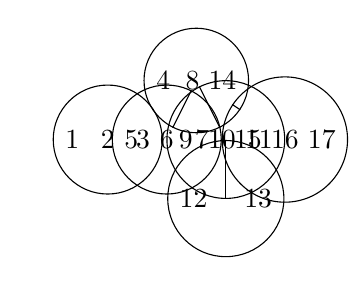
\begin{tikzpicture}[scale=0.5]

\node [circle,draw] (z){4\: 8 14}
  child {node [circle,draw] (a) {1\: \:2\: \:3}    
  }  
  child {node [circle,draw] (b) {5\: \:6\: \:7}
  }  
  child {node [circle,draw] (c) {9\: 10 11}
    child {node [circle,draw] (e) {12 \:\:\: 13}}
  }
  child {node [circle,draw] (d) {15 16 17}
  };

\end{tikzpicture}
\caption{Part 1. of ApproxMWPaging}
\end{subfigure}
\end{center}

\vspace{3em}

% Set the overall layout of the tree
\tikzstyle{level 1}=[level distance=3cm, sibling distance=3.5cm]
\tikzstyle{level 2}=[level distance=3cm, sibling distance=3.5cm]

\tikzset{smnode/.style={level 1/.style={level distance=1cm, sibling distance=1cm}, circle, draw}}
\tikzstyle{level 1}=[level distance=3cm, sibling distance=3.5cm]
\tikzstyle{level 2}=[level distance=3cm, sibling distance=3.5cm]
\tikzstyle{level 3}=[level distance=1cm, sibling distance=1cm]
\begin{center}
\begin{subfigure}[b]{0.82\textwidth}
\begin{tikzpicture}
\scriptsize
\node[circle,draw] (z){
	\tikzstyle{level 1}=[level distance=1cm, sibling distance=1cm]
	\begin{tikzpicture}
	\node [draw,circle] (zZ){8}
  	child {node [draw,circle] (Za) {4}    
  	}  
  	child {node [draw,circle] (Zb) {14}
  	};
	\end{tikzpicture}
}	
	  	
  child {node [circle,draw] (a) {
	\tikzstyle{level 2}=[level distance=1cm, sibling distance=1cm]
	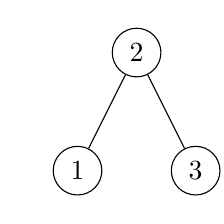
\begin{tikzpicture}
	\node [circle,draw] (z){2}
  	child {node [circle,draw] (a) {1}    
  	}  
  	child {node [circle,draw] (b) {3}
  	};
	\end{tikzpicture}  
  }edge from parent[shorten <=1.02cm] 
  }  
  child {node [circle,draw] (b) {
	\tikzstyle{level 2}=[level distance=1cm, sibling distance=1cm]
	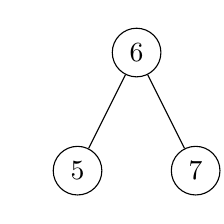
\begin{tikzpicture}
	\node [circle,draw] (z){6}
  	child {node [circle,draw] (a) {5}    
  	}  
  	child {node [circle,draw] (b) {7}
  	};
	\end{tikzpicture}   
  }edge from parent[shorten <=1.02cm]
  } 
  child {node [circle,draw] (c) {
	\tikzstyle{level 2}=[level distance=1cm, sibling distance=1cm]
	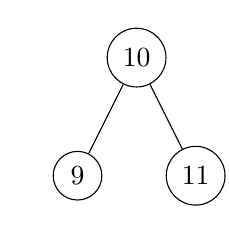
\begin{tikzpicture}
	\node [circle,draw] (z){10}
  	child {node [circle,draw] (a) {9}    
  	}  
  	child {node [circle,draw] (b) {11}
  	};
	\end{tikzpicture}  
  	}
  	child {node [circle,draw] (asdf) {
  	\tikzstyle{level 2}=[level distance=1cm, sibling distance=1cm]
	\begin{tikzpicture} 
	  	\node [smnode] (zz){12}
	  	child {node [circle,draw=none] {}edge from parent[draw=none]}	  	
  		child {node [smnode] (asaa) {13}    
  		}; 		
	\end{tikzpicture}	
  	}
  	}  	    
  edge from parent[shorten <=0.97cm]
  }
  child {node [circle,draw] (d) {
	\tikzstyle{level 2}=[level distance=1cm, sibling distance=1cm]
	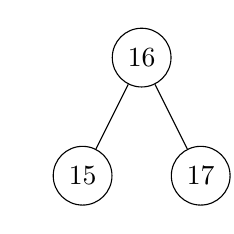
\begin{tikzpicture}
	\node [circle,draw] (z){16}
  	child {node [circle,draw] (a) {15}    
  	}  
  	child {node [circle,draw] (b) {17}
  	};
	\end{tikzpicture}   
  }edge from parent[shorten <=0.97cm]
  };
\end{tikzpicture}
\caption{Part 2. of ApproxMWPaging}
\end{subfigure}
\end{center}

\end{figure}

\clearpage

\begin{figure}[H]
\begin{center}
\scriptsize

\tikzstyle{level 1}=[level distance=1cm]
\tikzstyle{level 2}=[level distance=1cm]
\tikzstyle{level 3}=[level distance=1cm]
\begin{subfigure}[b]{0.72\textwidth}

\begin{tikzpicture}[level/.style={sibling distance=60mm/#1}]
\node [circle,draw] (z){8}
  child {node [circle,draw] (a) {4}    
	child {node [circle,draw] (b) {2}
		child {node [circle,draw] (c) {1}}
		child {node [circle,draw] (d) {3}}}  
  	child {node [circle,draw] (e) {6}
		child {node [circle,draw] (f) {5}}
		child {node [circle,draw] (g) {7}}}  
  }  
  child {node [circle,draw] (h) {14}    
	child {node [circle,draw] (i) {10}
		child {node [circle,draw] (j) {9}}
		child {node [circle,draw] (k) {11}
			child {node [circle,draw=none] (o) {}edge from parent[draw=none]}
			child {node [circle,draw] (o) {12}
				child {node [circle,draw=none] (s) {}edge from parent[draw=none]}				
				child {node [circle,draw] (p) {13}
		}}}}  
  	child {node [circle,draw] (l) {16}
		child {node [circle,draw] (m) {15}}
		child {node [circle,draw] (n) {17}}}  
  };

\end{tikzpicture}
\caption{Part 3. of ApproxMWPaging}



\end{subfigure}
\end{center}


\begin{center}
\scriptsize

\begin{subfigure}[b]{0.72\textwidth}


\begin{center}
    \begin{tabular}{ | l | l | l | p{5cm} |}
    \hline
    Memory Location & Node & Left Child Location & Right Child Location \\ \hline
    1  & 8  & 2    & 3    \\ \hline
    2  & 4  & 4    & 5    \\ \hline
    3  & 14 & 6    & 7    \\ \hline
    4  & 2  & 8    & 9    \\ \hline
    5  & 6  & 10   & 11   \\ \hline
    6  & 10 & 12   & 13   \\ \hline
    7  & 16 & 14   & 15   \\ \hline
    8  & 1  & --- & --- \\ \hline
    9  & 3  & --- & --- \\ \hline
    10 & 5  & --- & --- \\ \hline
    11 & 7  & --- & --- \\ \hline
    12 & 9  & --- & --- \\ \hline
    13 & 11 & --- & 16   \\ \hline
    14 & 15 & --- & --- \\ \hline
    15 & 17 & --- & --- \\ \hline
    16 & 12 & --- & 17   \\ \hline
    17 & 13 & --- & --- \\ \hline
    \end{tabular}
\end{center}

\caption{Part 4. of ApproxMWPaging}
\end{subfigure}
\end{center}


\caption{An example of the ApproxMWPaging algorithm.}
\end{figure}


\section{Expected Cost ApproxMWPaging} \label{45}

First, we bound the depth of nodes in our BST $T$. The depth of a key $B_i$ (or $(B_{i-1}, B_i)$ for gaps) is defined as $d_T(B_i)$ (resp. $d_T((B_{i-1},B_i))$). Note that depth is the number of edges between a node and the root (i.e. the depth of the root is $0$). As in the work of Bose and Dou\"{i}eb, let $m=\max({n-3P,P})-1 \geq \frac{n}{4} - 1$ where $P$ is the number of increasing or decreasing sequences in a left-to-right read of the access probabilities of the leaves (gaps) \cite{bose2009efficient}.

\begin{lem} \label{451}
For a key $B_i$,
\begin{align*} 
d_T(B_i) \leq \lg(\frac{1}{p_i}).
\end{align*}
For a key $(B_{i-1},B_i)$,
\begin{align*} 
d_T((B_{i-1},B_i)) \leq \lg(\frac{1}{q_i}) + 2
\end{align*}
for all gaps, and
\begin{align*} 
d_T((B_{i-1},B_i)) \leq \lg(\frac{1}{q_i}) + 1
\end{align*}
for at least $m$ of them (and the two extremal gaps, $(B_0, B_1)$ and $(B_n, B_{n+1})$). 
  
\end{lem}

\begin{proof}
First we note that in the tree $T'$ we build using Bose and Dou\"{i}eb's multiway tree algorithm, the maximum depth of keys (call this $d_{T'}(B_i), d_{T'}(B_{i-1},B_i)$) for a page size $m_1$ is \cite{bose2009efficient}:
\begin{align*} d_{T'}(B_i) &\leq \lfloor log_{m_1}(\frac{1}{p_i}) \rfloor \\
d_{T'}(B_{i-1},B_i) &\leq \lfloor log_{m_1}(\frac{2}{q_i}) \rfloor + 1 \text{ for all gaps, and}\\
d_{T'}(B_{i-1},B_i) &\leq \lfloor log_{m_1}(\frac{1}{q_i}) \rfloor + 1 \text{ for at least $m$ of them (and the two extremal gaps)}
 \end{align*}
As explained in the paper, these follow from Lemmas 1 and 2 of Bose and Dou\"{i}eb \cite{bose2009efficient}.

Inside a page, we make a balanced (ignoring weight) BST, so each key has a depth within a page of at most $\lfloor \lg(m_1) \rfloor$. Since our algorithm always connects the root of the BST made for a page to a key in the BST made for the page's parent, a key $B_i$ has a \textit{page depth} (the number of unique pages accessed in order to access the key) of at most the bounds on $d_{T'}(B_i)$ and $d_{T'}(B_{i-1},B_i)$ described. Since we examine at most $\lceil \lg(m_1) \rceil$ keys within any one page, (and only 1 gap in a leaf page) a key's depth is at most
\begin{align*}
d_T(B_i) &\leq \lfloor \lg(m_1) \rfloor \lfloor log_{m_1}(\frac{1}{p_i}) \rfloor \\
\implies d_T(B_i) &\leq \lg(m_1)\cdot log_{m_1}(\frac{1}{p_i}) \\
\implies d_T(B_i) &\leq \lg(\frac{1}{p_i}). \\
\end{align*}

\noindent For an unsuccessful search
\begin{align*}
d_T((B_{i-1},B_i)) &\leq \lfloor \lg(m_1) \rfloor \lfloor log_{m_1}(\frac{2}{q_i}) \rfloor + 1 \\
\implies d_T((B_{i-1},B_i)) &\leq \lg(m_1)\cdot log_{m_1}(\frac{2}{q_i}) + 1 \\
\implies d_T((B_{i-1},B_i)) &\leq \lg(\frac{1}{q_i}) + 2 \text{ for all gaps, and} \\
\implies d_T((B_{i-1},B_i)) &\leq \lg(\frac{1}{q_i}) + 1 \text{ for at least $m$ of them (and the two extremal gaps)}.
\end{align*}


\end{proof}

Next, we bound the cost of search for each key and each gap. Let $m'_j = \sum_{k \leq j} m_j$. We define $m'_0 = 0$.

\begin{lem} \label{locationLem}

For any key $B_i$, if
\begin{align*}
k=&min_{j \in \{1, ..., h\}} \mid m'_j \geq location(B_i) \text{ then} \\
&k=min_{j \in \{1, ..., h\}} \mid m'_j \geq \frac{2}{p_i}-1.
\end{align*}
Let $par(B_{i-1}, B_i)$ represent the parent of the node for gap $(B_{i-1}, B_i)$ in $T$. If $n \geq 1$, then for any gap $(B_{i-1}, B_i)$, if 
\begin{align*}
k=&min_{j \in \{1, ..., h\}} \mid m'_j \geq location(par(B_{i-1}, B_i)) \text{ then} \\
&k=min_{j \in \{1, ..., h\}} \mid m'_j \geq \lfloor \frac{4}{q_i}-\frac{1}{2} \rfloor \text{ and} \\
&k=min_{j \in \{1, ..., h\}} \mid m'_j \geq \lfloor \frac{2}{q_i}-\frac{1}{2} \rfloor \text{ for at least $m$ of them (and the two extremal gaps)}.
\end{align*}

\end{lem}

\begin{proof}
Knowing a key's depth, its location in $T$ (since we use a BFS to place nodes into memory) can be bounded as follows:

\begin{align*}
location(B_i) \leq 2^{d_T(B_i)+1}-1.
\end{align*}

From \ref{451} we know that $d_T(B_i) \leq \lg(\frac{1}{p_i})$. Thus,

\begin{align*}
location(B_i) &\leq 2^{\lg(\frac{1}{p_i})+1}-1 \\
location(B_i) &\leq 2^{\lg(\frac{2}{p_i})}-1 \\
location(B_i) &\leq \frac{2}{p_i}-1.
\end{align*}

A gap's location can be bounded as follows:

\begin{align*}
location(B_{i-1}, B_i) \leq 2^{d_T((B_{i-1},B_i))+1}-1.
\end{align*}

Because we placed our tree $T$ into memory in BFS order, we can also bound the depth of a gap's parent (we assume for the remainder of this proof that the tree is non-trivial, i.e. $n>0$).

\begin{align*}
location(par(B_{i-1}, B_i)) &\leq \lfloor \frac{location(B_{i-1}, B_i)}{2} \rfloor \\
location(par(B_{i-1}, B_i)) &\leq \lfloor \frac{2^{d_T((B_{i-1},B_i))+1}-1}{2} \rfloor \\
location(par(B_{i-1}, B_i)) &\leq \lfloor 2^{d_T((B_{i-1},B_i))}-\frac{1}{2} \rfloor
\end{align*}

Thus, for any gap $(B_{i-1},B_i)$,
\begin{align*}
location(par(B_{i-1},B_i)) &\leq \lfloor 2^{\lg(\frac{1}{q_i}) + 2}-\frac{1}{2} \rfloor \text{ using \ref{451}} \\
location(par(B_{i-1},B_i)) &\leq \lfloor \frac{4}{q_i}-\frac{1}{2} \rfloor \text{ for all gaps.}
\end{align*}
Moreover, a similar explanation shows that 
\begin{align*}
location(par(B_{i-1},B_i)) &\leq \lfloor \frac{2}{q_i}-\frac{1}{2} \rfloor \text{ for at least $m$ (and the two extremal) gaps.}
\end{align*}

\end{proof}


\begin{lem} \label{AMWPExactLem}
The cost of searching for key $B_i$ or gap $(B_{i-1},B_i)$, $(C(B_i) \text{ and } C(B_{i-1},B_i)$ respectively) can be bounded as follows: 
\begin{align*} 
C(B_i) \leq  \sum_{k'=1}^{k-1} &\left(\lfloor \lg(m'_{k'}+1) \rfloor - \lfloor \lg(m'_{k'-1}+1) \rfloor \right)\cdot c_{k'}+ 
 \left(\lg(\frac{1}{p_i}) + 1 - \lfloor \lg(m'_{k-1}+1) \rfloor \right)\cdot c_k\\
&\text{such that } \left( k=min_{j \in \{1, ..., h\}} \mid m'_j \geq \frac{2}{p_i}-1 \right) 
\end{align*}
\begin{align*}
C(B_{i-1},B_i) \leq \sum_{k'=1}^{k-1} &\left(\lfloor \lg(m'_{k'}+1) \rfloor - \lfloor \lg(m'_{k'-1}+1) \rfloor \right)\cdot c_{k'}+ 
\left(lg(\frac{1}{q_i}) + 2 - \lfloor \lg(m'_{k-1}+1) \rfloor \right)\cdot c_k \\
&\text{such that } \left( k=min_{j \in \{1, ..., h\}} \mid m'_j \geq \lfloor \frac{4}{q_i}-\frac{1}{2} \rfloor \right) \\
& \text{for all gaps, and}
\end{align*}
\begin{align*}
C(B_{i-1},B_i) \leq \sum_{k'=1}^{k-1} &\left(\lfloor \lg(m'_{k'}+1) \rfloor - \lfloor \lg(m'_{k'-1}+1) \rfloor \right)\cdot c_{k'}+ 
\left(lg(\frac{1}{q_i}) + 1 - \lfloor \lg(m'_{k-1}+1) \rfloor \right)\cdot c_k \\
&\text{such that } \left( k=min_{j \in \{1, ..., h\}} \mid m'_j \geq \lfloor \frac{2}{q_i}-\frac{1}{2} \rfloor \right) \\
 & \text{ for at least $m$ (and the two extremal) gaps}.
\end{align*}

\end{lem}


\begin{proof}
Consider accessing each key along the path from the root to key $B_i$. We will examine $d_T(B_i)$ keys. We access one key at depth $0$, one key at depth $1$, and so on. Because the tree is packed into memory in BFS order, a key a depth $j$ will be at memory index at most $2^j-1$. Now, consider how many levels of the binary search tree $T$ will fit in $m_1$. In order for all keys of depth $j$ (and higher) to be in $m_1$ we need:
\begin{align*}
2^{j+1}-1 \leq m_1 \implies j \leq \lg(m_1 + 1)-1.
\end{align*}
Thus, at least $\lfloor \lg(m_1 + 1) \rfloor$ levels of $T$ (since the root node has depth $0$) will completely fit on $m_1$. We expand this concept for arbitrary memory level $m_k$. The last level of $T$ to completely fit on $m_k$ or higher memories is the maximum $s$ such that:
\begin{align*}
2^s-1 \leq m'_k \implies s \leq \lg(m'_k + 1).
\end{align*}
Thus, at least $\lfloor \lg(m'_j + 1) \rfloor$ levels of $T$ fit on $m_j$ or higher levels of memory.
On our search for $B_i$, we make at least $\lfloor \lg(m_1 + 1) \rfloor$ checks for elements located at memory $m_1$. This costs a total of
\begin{align*}
\lfloor \lg(m_1 + 1) \rfloor \cdot c_1.
\end{align*}

Let $k$ be the minimum memory level such that $m'_k \geq location(B_i)$. For each memory level $m_k'$ for $0 < k' < k$, we make at least $\lfloor \lg(m'_{k'} + 1) \rfloor$ checks in $m'_{k'}$ or higher memories. Of these checks, at least $\lfloor \lg(m'_{k'-1} + 1) \rfloor$ are in memory levels strictly higher up in the memory hierarchy than $k'$. Since $c_\alpha > c_\beta$ for $\alpha > \beta$, an upper bound on the cost of searching for all elements in memory level $0 < k' < k$ on the path from the root to $B(i)$ is:
\begin{align*}
(\lfloor \lg(m'_{k'} + 1) \rfloor - \lfloor \lg(m'_{k'-1} + 1) \rfloor) \cdot c_k'.
\end{align*}
Finally, we can upper bound the cost of search within $m_k$ by assuming that all remaining searches take place at memory level $k$. The searches at level $k$ will cost at most:

\begin{align*}
(\lg(\frac{1}{p_i}) + 1 - \lfloor \lg(m'_{k-1}+1) \rfloor)\cdot c_k.
\end{align*}

Combining the above three equations (and summing over every memory level) gives us the total cost of searching for a key in the deepest part of the tree:

\begin{align*}
C(B_i) \leq &\sum_{k'=1}^{k-1} \left(\lfloor \lg(m'_{k'}+1) \rfloor - \lfloor \lg(m'_{k'-1}+1) \rfloor \right)\cdot c_{k'}+ \\
 &\left(\lg(\frac{1}{p_i}) + 1 - \lfloor \lg(m'_{k-1}+1) \rfloor \right)\cdot c_k \\
&\text{such that } \left( k=min_{j \in \{1, ..., h\}} \mid m'_j \geq location(B_i) \right)
\end{align*}

Similarly, to search for a gap $(B_{i-1},B_i)$ we must access each of its descendants in turn (but not the leaf node representing that gap itself). Our search effectively ends at the parent of $(B_{i-1},B_i)$. Thus, 

\begin{align*}
C(B_{i-1},B_i) \leq \sum_{k'=1}^{k-1} &\left(\lfloor \lg(m'_{k'}+1) \rfloor - \lfloor \lg(m'_{k-1}+1) \rfloor \right)\cdot c_{k'}+ \\
 &\left(lg(\frac{1}{q_i}) + 2 - \lfloor \lg(m'_{k-1}+1) \rfloor \right)\cdot c_k \\
&\text{such that } \left( k=min_{j \in \{1, ..., h\}} \mid m'_j \geq location(par(B_{i-1},B_i)) \right)
\end{align*}

For all gaps, and,  

\begin{align*}
C(B_{i-1},B_i) \leq \sum_{k'=1}^{k-1} &\left(\lfloor \lg(m'_{k'}+1) \rfloor - \lfloor \lg(m'_{k-1}+1) \rfloor \right)\cdot c_{k'}+ \\
&\left(lg(\frac{1}{q_i}) + 1 - \lfloor \lg(m'_{k-1}+1) \rfloor \right)\cdot c_k \\
&\text{such that } \left( k=min_{j \in \{1, ..., h\}} \mid m'_j \geq location(par(B_{i-1},B_i)) \right)
\end{align*}

for at least $m$ (and the two most extremal) gaps.

Plugging in our upper bounds on $location(B_i)$ and $location(par(B_{i-1},B_i))$ from \ref{locationLem} immediately gives us the desired result.

\end{proof}

In order to use \ref{AMWPExactLem}, we define a function $C'$, which consumes a key $B_i$ as follows:
\begin{align*}
C'(B_i) :=  \sum_{k'=1}^{k-1} &\left(\lfloor \lg(m'_{k'}+1) \rfloor - \lfloor \lg(m'_{k'-1}+1) \rfloor \right)\cdot c_{k'}+ \\
 &\left(\lg(\frac{1}{p_i}) + 1 - \lfloor \lg(m'_{k-1}+1) \rfloor \right)\cdot c_k\\
&\text{such that } \left( k=min_{j \in \{1, ..., h\}} \mid m'_j \geq \frac{2}{p_i}-1 \right) 
\end{align*}

We also define a function $C''$, which consumes a gap $(B_{i-1},B_i)$. First, we define:
\begin{align*}
Q = \{q_i : q_i \text{ among smallest }m \text{ gaps excluding the extremal gaps} \} \cup \{q_0, q_n\}
\end{align*}

\begin{align*}
C''((B_{i-1},B_i)) :=
\begin{cases}
\sum_{k'=1}^{k-1} &\left(\lfloor \lg(m'_{k'}+1) \rfloor - \lfloor \lg(m'_{k'-1}+1) \rfloor \right)\cdot c_{k'} + \\
 &\left(lg(\frac{1}{q_i}) + 2 - \lfloor \lg(m'_{k-1}+1) \rfloor \right)\cdot c_k \hspace{70pt} \text{ if } q_i \not\in Q \\
&\text{such that } \left( k=min_{j \in \{1, ..., h\}} \mid m'_j \geq \lfloor \frac{4}{q_i}-\frac{1}{2} \rfloor \right) \\ \\
\sum_{k'=1}^{k-1} &\left(\lfloor \lg(m'_{k'}+1) \rfloor - \lfloor \lg(m'_{k'-1}+1) \rfloor \right)\cdot c_{k'}+ \\
&\left(lg(\frac{1}{q_i}) + 1 - \lfloor \lg(m'_{k-1}+1) \rfloor \right)\cdot c_k \hspace{70pt} \text{ otherwise}\\
&\text{such that } \left( k=min_{j \in \{1, ..., h\}} \mid m'_j \geq \lfloor \frac{2}{q_i}-\frac{1}{2} \rfloor \right)
\end{cases}
\end{align*}

We can now bound the expected cost of search, $C$, in $T$ explicitly.

\begin{thm} \label{ExactApproxMWPagingThm}
\begin{align*}
C \leq \sum_{i=1}^{n} p_i\cdot  C'(B_i) + \sum_{i=1}^{n+1} q_i\cdot C''((B_{i-1},B_i)) 
\end{align*}

\end{thm}

\begin{proof}
The total expected cost of search is simply the sum of the weighted cost of search for all keys and gaps multiplied by their respective probabilities.
\begin{align*}
C &\leq \sum_{i=1}^{n} p_i\cdot C(B_i) + \sum_{j=1}^{n+1} q_j\cdot C(B_{i-1},B_i) 
\end{align*}

We note that functions $C'$ and $C''$ are exactly equal to the upper bounds of cost of search for a key or gap respectively as defined in \ref{AMWPExactLem}. Hence, we can simply plug them into the equation above and get an upper bound on the expected cost of search in $T$:
\begin{align*}
C &\leq \sum_{i=1}^{n} p_i\cdot C'(B_i) + \sum_{j=1}^{n+1} q_j\cdot C''((B_{i-1},B_i))
\end{align*}


\end{proof}


In order to get a more cleaner (albeit weaker) bound in terms of the entropy of the distribution, we now describe $W$, the cost of searching for a key located at the deepest node of tree $T$. As defined in Thite's work, we let $h$ be the smallest $j$ such that $m'_j \geq n$. Let $D(T)$ be the height of $T$ (the depth of the deepest node in the tree).

\begin{lem} \label{452}
\begin{align*}
W \leq \sum_{k=1}^{h-1} \left(\lfloor \lg(m'_k+1) \rfloor - \lfloor \lg(m'_{i-1}+1 \rfloor  \right)\cdot c_k+ \left(D(T) - \lfloor \lg(m'_{h-1}+1) \rfloor \right)\cdot c_h
\end{align*}
\end{lem}


\begin{proof}
We can follow the exact same logic as in \ref{AMWPExactLem} with the depth of our node as $D(T)$, and its memory level $h$. This immediately gives us the desired result.

\end{proof}

This leads us to the following upper bound for $W$.

\begin{lem} \label{W<HT}
Assuming that $l \neq 1$:
\begin{align*}
W<D(T)\cdot c_h
\end{align*}
\end{lem}

\begin{proof}
We can rearrange Lemma~\ref{452} as follows:
\begin{align*}
W \leq D(T)\cdot c_h - \sum_{k=1}^{h-1} \lfloor \lg(m'_k+1) \rfloor \cdot(c_{k+1} - c_k) 
\end{align*}
Since we have that $c_k > c_{k-1}$ for all $k$, $\sum_{k=1}^{h-1} \lfloor \lg(m'_k+1) \rfloor \cdot(c_{k+1} - c_k)$ is strictly positive. This instantly gives the result desired.
\end{proof}

Note that $\frac{W}{D(T)}$ represents the average cost per memory access when accessing the deepest (and most costly) element of our tree. Since our costs of access are monotonically increasing as we move deeper in the tree, we will see that $\frac{W}{D(T)}$ can be used as an upper bound for the average cost per memory access when searching for any element of $T$.

\begin{lem}
The cost of searching for a keys $B_i$ and $(B_{i-1},B_i)$ ($C(B_i)$ and $C((B_{i-1},B_i))$ respectively) can be bounded as follows: 
\begin{align*} 
C(B_i) &\leq (\lg(\frac{1}{p_i})+1)\cdot \frac{W}{D(T)} < (\lg(\frac{1}{p_i})+1)\cdot c_h \\
C((B_{i-1},B_i)) &\leq (\lg(\frac{1}{q_i})+2)\cdot \frac{W}{D(T)} < (\lg(\frac{1}{q_i})+2)\cdot c_h \text{ for all gaps, and} \\
C((B_{i-1},B_i)) &\leq (\lg(\frac{1}{q_i})+1)\cdot \frac{W}{D(T)} < (\lg(\frac{1}{q_i})+1)\cdot c_h \text{ for at least $m$ (and the two extremal) gaps}.
\end{align*}

\end{lem}

\begin{proof}
From Lemma~\ref{451} we have a bound on the depth of keys $B_i$ and $(B_{i-1},B_i)$. We must do $d_T(B_i) + 1$ accesses to find a key and $d_T((B_{i-1},B_i))$ accesses to find a gap. Note that since our tree is stored in BFS order in memory, whenever we examine a key's child, it will be at a memory location of at least the same, if not higher cost (by being in the same or a deeper page). Thus, the cost of accessing the entire path from the root to a specific key can be upper bounded by multiplying the length of this path by the average cost per memory access of the most expensive (and deepest) key of the tree (this is exactly $\frac{W}{D(T)}$). Note that when searching for keys, we must search along the entire path from root to the key in question, while we need only examine the path from the root to the parent of a key for unsuccessful $(B_{i-1},B_i)$ searches. Combining~\ref{451}, ~\ref{452} and~\ref{W<HT} gives
\begin{align*}
C(B_i) &\leq (\lg(\frac{1}{p_i})+1)\cdot\frac{W}{D(T)}\\
\implies C(B_i) &< (\lg(\frac{1}{p_i})+1)\cdot\frac{D(T)\cdot c_h}{D(T)}   \\
\implies C(B_i) &< (\lg(\frac{1}{p_i})+1)\cdot c_h
\end{align*}

For gaps we have that
\begin{align*}
C((B_{i-1},B_i)) &\leq (\lg(\frac{1}{q_i})+2)\cdot \frac{W}{D(T)}   \\
\implies C((B_{i-1},B_i)) &\leq (\lg(\frac{1}{q_i})+2)\cdot \frac{D(T)\cdot c_h}{D(T)}   \\
\implies C((B_{i-1},B_i)) &< (\lg(\frac{1}{q_i})+2)\cdot c_h \text{ for all gaps, and} \\
\implies C((B_{i-1},B_i)) &< (\lg(\frac{1}{q_i})+1)\cdot c_h \text{ for at least $m$ (and the two extremal) gaps}.
\end{align*}
\end{proof}

We can now bound the expected cost of search using the bounds for the cost each key.

\begin{thm} \label{ApproxMWPagingThm}
\begin{align*}
C &\leq  \frac{W}{D(T)} \cdot  \left(H + 1 + \sum_{i=0}^n q_i - q_0 - q_n - \sum_{i=0}^m q_{\text{rank}[i]} \right) \text{ and}\\
C &< \left(H + 1 + \sum_{i=0}^n q_i - q_0 - q_n - \sum_{i=0}^m q_{\text{rank}[i]} \right) \cdot  c_h
\end{align*}
where $q_{\text{rank}[i]}$ is the $i^{th}$ smallest access probability among gaps except $q_0$ and $q_n$.
\end{thm}

\begin{proof}
As in \ref{ExactApproxMWPagingThm}, the total expected cost of search is simply the sum of the weighted cost of search for all keys multiplied by the probability of searching for each key. Given our last lemma, we have that:
\begin{align*}
C &\leq \sum_{i=1}^{n} p_i\cdot C(B_i) + \sum_{j=1}^{n+1} q_j\cdot C((B_{i-1},B_i)) \\
\implies C &\leq \sum_{i=1}^{n} p_i\cdot (\lg(\frac{1}{p_i})+1)\cdot \frac{W}{D(T)} + \left(\sum_{i=0}^{n} q_i(\lg(\frac{1}{q_i})+2) - q_0 - q_n -  \sum_{i=0}^m q_{\text{rank}[i]} \right)\cdot \frac{W}{D(T)} \\
\implies C &\leq \frac{W}{D(T)} \left(\sum_{i=1}^{n} p_i\lg(\frac{1}{p_i}) + \sum_{i=0}^{n} q_i\lg(\frac{1}{q_i}) + \sum_{i=1}^{n} p_i + 2\sum_{i=0}^{n} q_i - q_0 - q_n - \sum_{i=0}^m q_{\text{rank}[i]} \right) \\
\implies C &\leq  \frac{W}{D(T)} \left(H + 1 + \sum_{i=0}^n q_i - q_0 - q_n - \sum_{i=0}^m q_{\text{rank}[i]} \right)
\end{align*}
By Lemma~\ref{W<HT} this gives:
\begin{align*}
C < \left(H + 1 + \sum_{i=0}^n q_i - q_0 - q_n - \sum_{i=0}^m q_{\text{rank}[i]} \right) \cdot  c_h
\end{align*}

\end{proof}


\section{Approximate Binary Search Trees of De Prisco and De Santis with Extensions by Bose and Dou\"{i}eb} \label{sec:deBST}

We provide another approach to building the approximately optimal BST under the HMM model. This approach uses the approximate BST solution (in the simple RAM model) of De Prisco and De Santos (modified by Bose and Dou\"{i}eb) \cite{de1993binary, bose2009efficient}. we explain the method here.

As in the classic Knuth problem, we are given a set of $n$ probabilities of searching for keys ($p_1, p_2, ..., p_n$), as well as $n+1$ probabilities of unsuccessful searches ($q_0, q_1, ..., q_n$). De Prisco and De Santos give an algorithm which constructs a binary search tree in $O(n)$ time with an expected cost of at most \cite{de1993binary}
\begin{align*}
H+1-q_0-q_n+q_{max}
\end{align*}
  where $q_{max}$ is the maximum probability of an unsuccessful search. This was later modified by Bose and Dou\"{i}eb (the same paper described in section~\ref{43}) to have an improved bound of \cite{bose2009efficient}
\begin{align*}
H + 1 - q_0 - q_n + q_{max} - \sum_{i=0}^{m'} pq_{\text{rank}[i]}.
\end{align*}
Here, $P$ is the number of increasing or decreasing sequences in a left-to-right read of the access probabilities of the gaps and $m'=\max({2n-3P,P})-1 \geq \frac{n}{2} - 1$.  Moreover, $pq_{\text{rank}[i]}$ is the $i^{th}$ smallest access probability among all keys and gaps except $q_0$ and $q_n$.

First, we a high level explanation of the algorithm of De Prisco and De Santis and then explain the extensions of Bose and Dou\"{i}eb. De Prisco and De Santis' algorithm occurs in three phases.

\begin{itemize}
\item[\textbf{Phase 1}] An auxiliary probability distribution is created using $2n$ zero probabilities, along with the $2n+1$ successful and unsuccessful search probabilities. Yeung's linear time alphabetic search tree algorithm is used with the $2n+1$ successful and unsuccessful search probabilities used as gaps of the new tree created \cite{yeung1991alphabetic}. This is referred to as the \textit{starting tree}.

\item[\textbf{Phase 2}] What's known as the \textit{redundant tree} is created by moving $p_i$ keys up the \textit{starting tree} to the lowest common ancestor of keys $q_{i-1}$ and $q_i$. The keys which used to be called $p_i$ are relabelled to $old.p_i$.

\item[\textbf{Phase 3}] The \textit{derived tree} is constructed from the \textit{redundant tree} by removing redundant edges. Edges to and from nodes which represented zero probability keys are deleted. This \textit{derived tree} is a binary search tree with the expected search cost described.
\end{itemize}


In Bose and Dou\"{i}eb's work, they explain how they can substitute their algorithm for Yeung's linear time alphabetic search tree algorithm which results in a better bound (as described above). We use the updated version (by Bose and Dou\"{i}eb) of De Prisco and De Santis' algorithm as a subroutine in the sections to follow.

Let $T_1$ be the \textit{starting tree} created after \textbf{Phase 1} of the algorithm using Bose and Dou\"{i}eb's method. As explained Section 4 of their work \cite{bose2009efficient}, every leaf (both keys and gaps from the original dataset) with probability $\alpha$ have depth at most:
\begin{align*}
d_{T_1}(\alpha) \leq
\begin{cases}
\lfloor \lg \frac{1}{\alpha} \rfloor + 1 \text{ for at least } \max\{2n-3P\}-1 \text{ and the extremal gaps of } T_1 \\
\lfloor \lg \frac{1}{\alpha} \rfloor + 2 \text{ otherwise}
\end{cases}
\end{align*}

Moreover, each key from our original data set has its depth decreased by at least $2$ while each leaf from our original data set, except for possibly one, has its depth reduced by at least $1$ in the next two phases of the algorithm. We wish to write this out as an explicit Lemma for use in \ref{48}. First, we define $R$:

\begin{align*}
R = \{\alpha : \alpha &\text{ among the }m' \text{ smallest access probabilities for keys or gaps excluding the} \\
&\text{ extremal gaps} \} \cup \{q_0, q_n\} - \{q_{max}\}
\end{align*}

\begin{lem} \label{ApprBSTLem}

Let $T$ be a tree made using the approximate binary search tree algorithm of De Prisco and De Santis with extensions by Bose and Dou\"{i}eb. For a key $B_i$,
\begin{align*} 
d_T(B_i) \leq
\begin{cases}  
\lfloor \lg(\frac{1}{p_i}) \rfloor - 1 &\text{ if } p_i \in R  \\
\lfloor \lg(\frac{1}{p_i}) \rfloor &\text{ otherwise.}
\end{cases}
\end{align*}

For a gap $(B_{i-1},B_i)$,
\begin{align*}
d_T((B_{i-1},B_i)) \leq
\begin{cases}  
\lfloor \lg(\frac{1}{q_i}) \rfloor &\text{ if } q_i \in R  \\
\lfloor \lg(\frac{1}{q_i}) \rfloor + 2 &\text{ if } q_i \text{ is } q_{max} \\
\lfloor \lg(\frac{1}{p_i}) \rfloor + 1 &\text{ otherwise.}
\end{cases}
\end{align*}
  
\end{lem}

\begin{proof}
This follows directly from the explanation above.
\end{proof}

\section{Algorithm ApproxBSTPaging}\label{Algorithm ApproxBSTPaging}

Our second solution to create an approximately optimal BST under the HMM model works as follows: \\

\begin{enumerate}
\item First, we create a BST $T$ using the algorithm of De Prisco and De Santis \cite{de1993binary} (as updated by Bose and Dou\"{i}eb \cite{bose2009efficient}). This takes $O(n)$ time. \\

\item In a similar fashion to step 4) of \ref{Algorithm ApproxMWPaging}, we pack keys from $T$ into memory in a breadth-first search order starting from the root. This relatively simple traversal also takes $O(n)$ time.
\end{enumerate}

We are left with a binary search tree which is properly packed into memory in total time $O(n)$.


\section{Expected Cost ApproxBSTPaging}\label{48}

The explanation here follows in a similar manner to that of \ref{45}. First, we use \ref{ApprBSTLem} to bound the depth of a node in the memory hierarchy given its probability. The proof follows in a similar fashion to \ref{locationLem}. Recall that $m'_j = \sum_{k \leq j} m_j$ and $m'_0 = 0$. Moreover, recall $R$:

\begin{align*}
R = \{\alpha : \alpha &\text{ among the }m' \text{ smallest access probabilities for keys or gaps excluding the} \\
&\text{ extremal gaps} \} \cup \{q_0, q_n\} - \{q_{max}\}
\end{align*}

\begin{lem} \label{locationLemBST}

For any key $B_i$, if
\begin{align*}
k=&min_{j \in \{1, ..., h\}} \mid m'_j \geq location(B_i) \text{ then} \\
&k=min_{j \in \{1, ..., h\}} \mid m'_j \geq \frac{1}{p_i}-1 \text{ if } p_i \in R \\
&k=min_{j \in \{1, ..., h\}} \mid m'_j \geq \frac{2}{p_i}-1 \text{ otherwise.}
\end{align*}
Let $par(B_{i-1}, B_i)$ represent the parent of the node for gap $(B_{i-1}, B_i)$ in $T$. If $n \geq 1$, then for any gap $(B_{i-1}, B_i)$, if 
\begin{align*}
k=&min_{j \in \{1, ..., h\}} \mid m'_j \geq location(par(B_{i-1}, B_i)) \text{ then} \\
&k=min_{j \in \{1, ..., h\}} \mid m'_j \geq \lfloor \frac{1}{q_i}-\frac{1}{2} \rfloor \text{ if } q_i \in R \\
&k=min_{j \in \{1, ..., h\}} \mid m'_j \geq \lfloor \frac{4}{q_i}-\frac{1}{2} \rfloor \text{ else if } q_i = q_{max} \\
&k=min_{j \in \{1, ..., h\}} \mid m'_j \geq \lfloor \frac{2}{q_i}-\frac{1}{2} \rfloor \text{ otherwise}.
\end{align*}

\end{lem}

\begin{proof}
As before, knowing a key's depth, its location in $T$ can be bounded as follows:

\begin{align*}
location(B_i) \leq 2^{d_T(B_i)+1}-1.
\end{align*}

Hence, using \ref{ApprBSTLem} we get:

\begin{align*}
location(B_i) &\leq 2^{\lfloor \lg(\frac{1}{p_i}) \rfloor -1 +1}-1 \\
location(B_i) &\leq 2^{\lg(\frac{1}{p_i})}-1 \\
location(B_i) &\leq \frac{1}{p_i}-1 \text{ when } p_i \in R  \text{ and}
\end{align*}

\begin{align*}
location(B_i) &\leq 2^{\lfloor \lg(\frac{1}{p_i}) \rfloor +1}-1 \\
location(B_i) &\leq 2^{\lg(\frac{2}{p_i})}-1 \\
location(B_i) &\leq \frac{2}{p_i}-1 \text{ otherwise.}
\end{align*}


Recall a gap's location and its parent's location can be bounded as follows:

\begin{align*}
location(B_{i-1}, B_i) &\leq 2^{d_T((B_{i-1},B_i))+1}-1 \\
location(par(B_{i-1}, B_i)) &\leq \lfloor 2^{d_T((B_{i-1},B_i))}-\frac{1}{2} \rfloor
\end{align*}

Thus, for any gap $(B_{i-1},B_i)$,
\begin{align*}
location(par(B_{i-1},B_i)) &\leq \lfloor 2^{\lg(\frac{1}{q_i})}-\frac{1}{2} \rfloor& \\
location(par(B_{i-1},B_i)) &\leq \lfloor \frac{1}{q_i}-\frac{1}{2} \rfloor &\text{ if } q_i \in R 
\end{align*}
\begin{align*}
location(par(B_{i-1},B_i)) &\leq \lfloor 2^{\lg(\frac{1}{q_i}) + 2}-\frac{1}{2} \rfloor& \\
location(par(B_{i-1},B_i)) &\leq \lfloor \frac{4}{q_i}-\frac{1}{2} \rfloor &\text{ if } q_i = q_{max}
\end{align*}

\begin{align*}
location(par(B_{i-1},B_i)) &\leq \lfloor 2^{\lg(\frac{1}{q_i}) + 1}-\frac{1}{2} \rfloor& \\
location(par(B_{i-1},B_i)) &\leq \lfloor \frac{2}{q_i}-\frac{1}{2} \rfloor &\text{ otherwise.}
\end{align*}

\end{proof}

As in \ref{45} we can now bound the cost of search for keys and gaps.

\begin{lem} \label{ABSTExactLem}
The cost of searching for key $B_i$ or gap $(B_{i-1},B_i)$, $(C(B_i) \text{ and } C(B_{i-1},B_i)$ respectively) using the \textit{ApproxBSTPaging} algorithm can be bounded as follows: 
\begin{align*} 
C(B_i) \leq 
\begin{cases}
 \sum_{k'=1}^{k-1} &\left(\lfloor \lg(m'_{k'}+1) \rfloor - \lfloor \lg(m'_{k'-1}+1) \rfloor \right)\cdot c_{k'}+ \\
 &\left(\lg(\frac{1}{p_i}) - \lfloor \lg(m'_{k-1}+1) \rfloor \right)\cdot c_k\\
&\text{such that } k=min_{j \in \{1, ..., h\}} \mid m'_j \geq \frac{1}{p_i}-1 \text{ if } p_i \in R \\\\
 \sum_{k'=1}^{k-1} &\left(\lfloor \lg(m'_{k'}+1) \rfloor - \lfloor \lg(m'_{k'-1}+1) \rfloor \right)\cdot c_{k'}+ \\
 &\left(\lg(\frac{1}{p_i}) + 1 - \lfloor \lg(m'_{k-1}+1) \rfloor \right)\cdot c_k\\
&\text{such that } k=min_{j \in \{1, ..., h\}} \mid m'_j \geq \frac{2}{p_i}-1 \text{ otherwise.}  
\end{cases}
\end{align*}
\begin{align*}
C((B_{i-1},B_i)) \leq
\begin{cases}
 \sum_{k'=1}^{k-1} &\left(\lfloor \lg(m'_{k'}+1) \rfloor - \lfloor \lg(m'_{k'-1}+1) \rfloor \right)\cdot c_{k'}+ \\
 &\left(\lg(\frac{1}{q_i}) - \lfloor \lg(m'_{k-1}+1) \rfloor \right)\cdot c_k\\
&\text{such that } k=min_{j \in \{1, ..., h\}} \mid m'_j \geq \lfloor \frac{1}{q_i}-\frac{1}{2} \rfloor \text{ if } q_i \in R  \\\\
  \sum_{k'=1}^{k-1} &\left(\lfloor \lg(m'_{k'}+1) \rfloor - \lfloor \lg(m'_{k'-1}+1) \rfloor \right)\cdot c_{k'}+ \\
 &\left(\lg(\frac{1}{q_i}) + 2 - \lfloor \lg(m'_{k-1}+1) \rfloor \right)\cdot c_k\\
&\text{such that } k=min_{j \in \{1, ..., h\}} \mid m'_j \geq \lfloor \frac{4}{q_i}-\frac{1}{2} \rfloor \text{ else if } q_i = q_{max}  \\\\
 \sum_{k'=1}^{k-1} &\left(\lfloor \lg(m'_{k'}+1) \rfloor - \lfloor \lg(m'_{k'-1}+1) \rfloor \right)\cdot c_{k'}+ \\
 &\left(\lg(\frac{1}{q_i})+1 - \lfloor \lg(m'_{k-1}+1) \rfloor \right)\cdot c_k\\
&\text{such that } k=min_{j \in \{1, ..., h\}} \mid m'_j \geq \lfloor \frac{2}{q_i}-\frac{1}{2} \rfloor \text{ otherwise.}
\end{cases}
\end{align*}
\end{lem}


\begin{proof}
The proof follows an almost identical set of logic to \ref{AMWPExactLem} in terms of how far into the tree we search for each node. We then can simply plug in the maximum depth of nodes from \ref{ApprBSTLem}, and the maximum location in the memory hierarchy from \ref{locationLemBST} and arrive at the result.
\end{proof}


In order to use \ref{ABSTExactLem}, we define a function $C'$, which consumes a key $B_i$ as follows:
\begin{align*} 
C'(B_i) := 
\begin{cases}
 \sum_{k'=1}^{k-1} &\left(\lfloor \lg(m'_{k'}+1) \rfloor - \lfloor \lg(m'_{k'-1}+1) \rfloor \right)\cdot c_{k'}+ \\
 &\left(\lg(\frac{1}{p_i}) - \lfloor \lg(m'_{k-1}+1) \rfloor \right)\cdot c_k\\
&\text{such that } k=min_{j \in \{1, ..., h\}} \mid m'_j \geq \frac{1}{p_i}-1 \text{ if } p_i \in R \\\\
 \sum_{k'=1}^{k-1} &\left(\lfloor \lg(m'_{k'}+1) \rfloor - \lfloor \lg(m'_{k'-1}+1) \rfloor \right)\cdot c_{k'}+ \\
 &\left(\lg(\frac{1}{p_i}) + 1 - \lfloor \lg(m'_{k-1}+1) \rfloor \right)\cdot c_k\\
&\text{such that } k=min_{j \in \{1, ..., h\}} \mid m'_j \geq \frac{2}{p_i}-1 \text{ otherwise.}  
\end{cases}
\end{align*}

We also define a function $C''$, which consumes a gap $(B_{i-1},B_i)$:

\begin{align*}
C''((B_{i-1},B_i)) :=
\begin{cases}
 \sum_{k'=1}^{k-1} &\left(\lfloor \lg(m'_{k'}+1) \rfloor - \lfloor \lg(m'_{k'-1}+1) \rfloor \right)\cdot c_{k'}+ \\
 &\left(\lg(\frac{1}{q_i}) - \lfloor \lg(m'_{k-1}+1) \rfloor \right)\cdot c_k\\
&\text{such that } k=min_{j \in \{1, ..., h\}} \mid m'_j \geq \lfloor \frac{1}{q_i}-\frac{1}{2} \rfloor \text{ if } q_i \in R  \\\\
  \sum_{k'=1}^{k-1} &\left(\lfloor \lg(m'_{k'}+1) \rfloor - \lfloor \lg(m'_{k'-1}+1) \rfloor \right)\cdot c_{k'}+ \\
 &\left(\lg(\frac{1}{q_i}) + 2 - \lfloor \lg(m'_{k-1}+1) \rfloor \right)\cdot c_k\\
&\text{such that } k=min_{j \in \{1, ..., h\}} \mid m'_j \geq \lfloor \frac{4}{q_i}-\frac{1}{2} \rfloor \text{ else if } q_i = q_{max}  \\\\
 \sum_{k'=1}^{k-1} &\left(\lfloor \lg(m'_{k'}+1) \rfloor - \lfloor \lg(m'_{k'-1}+1) \rfloor \right)\cdot c_{k'}+ \\
 &\left(\lg(\frac{1}{q_i})+1 - \lfloor \lg(m'_{k-1}+1) \rfloor \right)\cdot c_k\\
&\text{such that } k=min_{j \in \{1, ..., h\}} \mid m'_j \geq \lfloor \frac{2}{q_i}-\frac{1}{2} \rfloor \text{ otherwise.}
\end{cases}
\end{align*}

We can now bound the expected cost of search, $C$, in $T$ explicitly.

\begin{thm} \label{ExactApproxBSTPagingThm}
\begin{align*}
C \leq \sum_{i=1}^{n} p_i\cdot  C'(B_i) + \sum_{i=1}^{n+1} q_i\cdot C''((B_{i-1},B_i)) 
\end{align*}

\end{thm}

\begin{proof}
The total expected cost of search is simply the sum of the weighted cost of search for all keys and gaps multiplied by their respective probabilities.
\begin{align*}
C &\leq \sum_{i=1}^{n} p_i\cdot C(B_i) + \sum_{j=1}^{n+1} q_j\cdot C(B_{i-1},B_i) 
\end{align*}

As in \ref{ExactApproxMWPagingThm}, $C'$ and $C''$ are exactly equal to the upper bounds of cost of search for a key or gap respectively as defined in \ref{ABSTExactLem}. We simply plug them into the equation above and get an upper bound on the expected cost of search in $T$:
\begin{align*}
C &\leq \sum_{i=1}^{n} p_i\cdot C'(B_i) + \sum_{j=1}^{n+1} q_j\cdot C''((B_{i-1},B_i))
\end{align*}

\end{proof}




Like in \ref{45}, as wish to make a cleaner albeit weaker bound in terms of the entropy of the probability distribution. As explained in the Bose and Dou\"{i}eb paper, the average path length search cost of the tree created by their algorithm is at most: \cite{bose2009efficient}
\begin{align*}
H + 1 - q_0 - q_n + q_{max} - \sum_{i=0}^{m'} pq_{\text{rank}[i]}
\end{align*}

We call this value $P_T$ (the average search cost of tree $T$). Similar to the proof in section~\ref{45}, if we can bound the cost of search for a given path length, then we can form a bound on the average cost of search in the HMM model. As before, we can describe the cost of searching for a key located at deepest node of tree $T$: $W$. Recall, $m'_j = \sum_{k \leq j} m_k$, $m'_0 = 0$ and let $h$ be the smallest $j$ such that $m'_j \geq n$.

\begin{lem} 
When using the ApproxBSTPaging, the cost of searching for a node deepest in the tree is at most:
\begin{align*}
W \leq \sum_{k=1}^{h-1} \left(\lfloor \lg(m'_k+1) \rfloor - \lfloor \lg(m'_{i-1}+1) \rfloor)\cdot c_k+ (D(T) - \lfloor \lg(m'_{h-1}+1) \rfloor \right)\cdot c_h
\end{align*}
\end{lem}

\begin{proof}
Since we are simply putting keys into memory in BFS order, and all we use is the height of the tree and the memory hierarchy, the proof is identical to that of Lemma~\ref{452}.
\end{proof}

Since we have the same result as Lemma~\ref{452}, this immediately implies Lemma~\ref{W<HT} is true as well. Assuming that $l \neq 1$, we have that $W<D(T)\cdot c_h$. As in \ref{ExactApproxMWPagingThm}, $\frac{W}{D(T)}$ represents the average cost per memory access when accessing the deepest (and most costly) element of our tree. Thus, $\frac{W}{D(T)}$ upper bounds the average cost per memory access when searching for any element of $T$.
\\

\begin{thm} \label{ApproxBSTThm}
\begin{align*}
C &\leq  (\frac{W}{D(T)}) \cdot  (H + 1 - q_0 - q_n + q_{max} - \sum_{i=0}^{m'} pq_{\text{rank}[i]}) \text{ and} \\
C &<  (H + 1 - q_0 - q_n + q_{max} - \sum_{i=0}^{m'} pq_{\text{rank}[i]})\cdot c_h
\end{align*}
\end{thm}

\begin{proof}

Bose and Dou\"{i}eb show that after using their algorithm for Phase 1 of De Prisco and De Santis algorithm algorithm, every leaf of the \textit{starting tree} (all keys representing successful searches and gaps representing unsuccessful searhces) are at depth at most $\lfloor \lg(\frac{1}{p}) \rfloor + 1$  for at least $\max(2n-3P,P)-1$ of $p \in \left( \{p_1, p_2, ..., p_n \} \cup \{ q_0, q_1, ..., q_n \} \right)$ and $\lfloor \lg(\frac{1}{p}) \rfloor + 2$ for all others. Recall that $P$ is the number of peaks in the probability distribution $q_0, p_1, q_1, ..., p_n, q_n$. After phases 2 and 3 of the algorithm, each key has its depth decrease by 2, and all gaps (except one) move up the tree by one.
\begin{align*}
C &\leq \sum_{i=1}^{n} \left(p_i\cdot \frac{depth(p_i)+1}{D(T)}\cdot  W \right)+ \sum_{i=0}^{n} \left(q_i\cdot \frac{(depth(q_i))}{D(T)}\cdot  W \right) \\
\implies C &\leq \frac{W}{D(T)} \left(\sum_{i=1}^{n}(p_i\cdot (depth(p_i)+1))+ \sum_{i=0}^{n}(q_i\cdot (depth(q_i))) \right) \\
\implies C &\leq \frac{W}{D(T)} \left(\text{WeightedAveragePathLength}(T) \right) \\
\implies C &\leq  \left( \frac{W}{D(T)} \right) \cdot  \left(H + 1 - q_0 - q_n + q_{max} - \sum_{i=0}^{m'} pq_{\text{rank}[i]} \right) \text{ and by Lemma~\ref{W<HT}} \\
\implies C &<  \left(H + 1 - q_0 - q_n + q_{max} - \sum_{i=0}^{m'} pq_{\text{rank}[i]} \right)\cdot c_h
\end{align*}

\end{proof}


\section{Improvements over Thite in the HMM$_2$ Model}

The HMM$_2$ model is the same as the general HMM model with the added constraint that there are only two types of memory (slow and fast). In Thite's thesis, he proposed both an optimal solution to the problem, as well as an approximate solution (\textit{Algorithm Approx-BST}) that runs in time $O(n \lg(n))$ \cite{thite2008optimum}. we first show that:
\begin{lem}
The proof of quality of approximation of Thite's approximate algorithm has a small mistake which raises its cost from at most: 
\begin{align*}
&c_2(H+1) \text{ to} \\
&c_2(H+1+\sum_{i=0}^{n}q_i)
\end{align*}
\end{lem}

\begin{proof}
Specifically, in Lemma 14 in 3.4.2.3 Quality of approximation in Thite's thesis, he proves that $\delta(z_k) = l+2$. Here, $\delta(z_k)$ represents the depth of a leaf node $z_k$. Note that Thite considers the depth of the root to be $1$ instead of $0$ which updates how the cost of search is calculated accordingly. $l$ represents the depth of recursion of the \textit{Approx-BST} algorithm. In Lemma 15, Thite goes on to prove that $q_k \leq 2^{-\delta(z_k)+2}$. In this proof, Thite shows that $q_k \leq 2^{-l+1}$, but makes a mistake when substituting in $l=\delta(z_k)-2$ and gets $q_k \leq 2^{-\delta(z_k)+2}$ while the correct bound is $q_k \leq 2^{-\delta(z_k)+3}$. This updated bound would change his depth bound in Lemma 16 from $\delta(z_k) \leq \lfloor \lg(\frac{1}{q_k}) \rfloor + 2$ to $\delta(z_k) \leq \lfloor \lg(\frac{1}{q_k}) \rfloor + 3$. Finally, substituting into his final equation for the upper bound on the expected cost of search for the tree would give:

\begin{align*}
&\sum_{i=1}^{n} \left(c_2 p_i \delta(B_i )+ \sum_{i=0}^{n} c_2 q_i (\delta(q_i)-1) \right)\\
\leq &\sum_{i=1}^{n} \left(c_2 p_i (\lg(\frac{1}{p_i})+1)+ \sum_{i=0}^{n} c_2 q_i (\lg(\frac{1}{q_i})+3-1) \right) \\
\leq &c_2 \cdot \left(H+1+\sum_{i=0}^{n}q_i \right)
\end{align*}
\end{proof}

This is of particular interest because if Thite's bound on \textit{Algorithm Approx-BST} had been correct, then in the case where $c_2=c_1$ (typical RAM model), Thite's method would have provided a strict improvement over the work of Bose and Dou\"{i}eb \cite{bose2009efficient} which seems unlikely since Thite used the BST approximation algorithm of Mehlhorn from 1984 \cite{mehlhorn1984sorting} (much before the work of Bose and Dou\"{i}eb).

By simply substituting in for $l=2$ we immediately get that, under this HMM$_2$ model, both ApproxMWPaging and ApproxBSTPaging provide strict improvements over Thite's \textit{Algorithm Approx-BST}. 

\begin{thm}
In the HMM$_2$ model, ApproxMWPaging has an expected cost of at most \\
\begin{align*}
C_{ApproxMWPaging} < (H + 1 + \sum_{i=0}^n q_i - q_0 - q_n - \sum_{i=0}^m q_{\text{rank}[i]}) \cdot  c_2
\end{align*}
and ApproxBSTPaging has an expected cost of at most
\begin{align*}
C_{ApproxBSTPaging} <  (H + 1 - q_0 - q_n + q_{max} - \sum_{i=0}^{m'} pq_{\text{rank}[i]})\cdot c_2.
\end{align*}
ApproxMWPaging and ApproxBSTPaging do so in $O(n)$ time.
\end{thm}

\begin{proof}
We can directly sub $l=2$ into Theorems~\ref{ApproxMWPagingThm} and~\ref{ApproxBSTThm} to get the desired result (the running times are as explained in sections~\ref{Algorithm ApproxMWPaging} and~\ref{Algorithm ApproxBSTPaging}).
\end{proof}

Since both ApproxMWPaging and ApproxBSTPaging run in time $o(n\lg(n))$ (the time of Thite's \textit{Approx-BST} algorithm) and we can see that:\\
\begin{align*}
C_{ApproxMWPaging} &< (H + 1 + \sum_{i=0}^n q_i - q_0 - q_n - \sum_{i=0}^m q_{\text{rank}[i]}) \cdot  c_2 \\
&< c_2(H+1+\sum_{i=0}^{n}q_i) \\
 C_{ApproxBSTPaging} &< (H + 1 - q_0 - q_n + q_{max} - \sum_{i=0}^{m'} pq_{\text{rank}[i]})\cdot c_2 \\
 &< c_2(H+1+\sum_{i=0}^{n}q_i)
 \end{align*}

Both methods provide a strictly better approximation and run faster than the \textit{Algorithm Approx-BST} of Thite.

%=========================================
\chapter{Binary Trees On Unordered Sequences of Probabilities}\label{BST over Multisets}

In this chapter we examine a problem related to the initial optimal binary search tree problem of Knuth \cite{knuth1971optimum}. The $n$ keys (represented using simply their probabilities) provided will no longer have an ordering and can be rearranged as we please before constructing our binary tree. We also do not have any restrictions on which keys can be internal nodes and which keys can be leaves. This problem is very similar to constructing optimal prefix-free binary codes which is solved using a Huffman coding. The problem differs however because we must place the $n$ probabilities at internal \textit{and} leaf node positions and cannot add extra nodes. Moreover, when searching, our cost model charges $1$ for each internal node we examine but does not charge for leaf nodes (since we do not need to "examine" them). Under this cost model, we show that our $O(n \lg(n))$ time algorithm \textit{GREEDY-MS} is within$\frac{n+1}{2n}$ of optimal.

\section{The Binary Tree On Unordered Sequences of Probabilities Problem}\label{The Multiset Binary Search Tree Problem}

 Consider a multiset (a set with possible duplicate values) of $n$ probabilities: $M = \lbag p_1, p_2, ..., p_n \rbag$ such that $\sum\limits_{i=1}^n p_i = 1$. We assume $n$ is odd. Our goal is to create a binary tree $T$ which minimizes the expected search cost, $C_{T_S}$, of nodes. We call this cost model the  the \textit{\textbf{S}tandard Model} since it is standard among other optimal BST problems.
\begin{equation}
C_{T_S} = \sum_{i=1}^{n} p_i(b_i+1) - \sum_{i \in L_T}p_i
\end{equation}
Here, $b_i$ is the \emph{depth} of the $i$'th key of $M$ and $L_T$ is the set of leaves of $T$. We subtract the weight of the leaves of the tree since we need one less comparison to return a pointer a leaf node (as in the original optimal BST problem). Note that this is analogous to our previous cost model \ref{1.1} but with a simple modification of how we describe the set of leaves ($L_T$ instead of $\{q_i\}$ for appropriate $i$).

\section{The GREEDY-MS Algorithm is Within $\frac{n+1}{2n}$ of Optimal}\label{GREEDY-MS}

First, we consider a new cost model for this problem, the \textit{\textbf{E}xpected Path Length Model}, which has cost $C_{T_E}$ defined as follows:
\begin{equation}
C_{T_E} = \sum_{i=1}^{n} p_i(b_i+1)
\end{equation}

The model treats leaves and internal nodes the same, charging $1$ for each node that must be examined when searching through the tree from the root for a specific node. This model corresponds to the a problem under the \textit{Standard Model}, but with the addition of $n+1$ probabilities with value $0$, which should obviously be placed at $n+1$ leaf locations.

As described in \cite{golin2012huffman} there is a simple greedy $O(n \lg n)$ time algorithm which solves the problem optimally. We call this algorithm \textit{GREEDY-MS}:

\begin{enumerate}
\item First, we create a vector $R$ which is equal to the sorted (from largest to smallest) multiset $M$.

\item We create a BST $T$ as follows. The root of our tree will be $R[0]$, its two children will be $R[1]$ and $R[2]$, and so on. Formally, $R[i]$ will be placed at location $i+1$ in the BFS order of $T$.
\end{enumerate}

For completeness we formally prove its optimality under the \textit{Expected Path Length Model}. 

\begin{lem}\label{MSSolvesOpt}
The tree $T$ created by \textit{GREEDY-MS} for the multiset of probabilities $M$ solves the problem under the \textit{Expected Path Length Model} optimally.
\end{lem}

\begin{proof}
Let $T'$ be an optimal tree under the \textit{Expected Path Length Model}. \\\\
\noindent \textbf{Claim 1.}\label{Claim-EPL}
For a given depth $d$, the probabilities of all nodes on level $d+1$ are greater than or equal to the probabilities of all nodes on level $d$.
\begin{proof}
If Claim 1 were not true, suppose $p_i$ and $p_j$ were the two probabilities which contradicted the statement. Swap their positions. The cost of the resulting tree is strictly less, which contradicts the optimality of $T'$.
\end{proof}

\noindent \textbf{Claim 2.}\label{Claim-EPL2}
For a given depth $d$ strictly less than the height of $T'$, $T'$ must be full.
\begin{proof}
If Claim 2 were not true consider $d'$; the smallest depth where it is not true. Take a leaf node with depth strictly greater than $d'$ and place it at depth $d$ in $T'$. The resulting tree costs strictly less than $T'$, another contradiction.
\end{proof}

Taking claims 1 and 2 together means that all optimal trees are full (except at the greatest depth) and always have higher probabilities above lower probabilities. All such trees are identical to $T$ created by \textit{GREEDY-MS} up to permutations among probabilities at a given depth $d$, and amongst identical probabilities. This completes the proof.

\end{proof}

In order to prove that \textit{GREEDY-MS} is within $\frac{n+1}{2n}$ of optimal under the \textit{Standard Model}  we first we must prove a lemma for optimal trees under the \textit{Standard Model}. We show that for an optimal tree where, for each parent child relationship, the parent has probability at least as large as the child, each leaf node (except one, the minimum) has a unique corresponding internal node with probability at least as big.

We say a leaf $p_i$ is \textit{covered} by a unique internal node $p_i'$ if $p_i'$ is an internal node, $p_i$ is a leaf node and $p_i' \geq p_i$.

\begin{lem}\label{leavesCovered}
Let $T$ be an optimal tree under the \textit{Standard Model} such that, for all child parent pairs, the probability of the parent is greater than that of the child. Let $l_{min}$ be the smallest leaf node by probability.
\begin{align*}
\forall_{p_i \in L_T-\{l_{min}\}} \exists \text{ unique } p_i' \notin \{L_T \cup \{l_{min}\}\} \text{ such that } p_i' \text{ covers } p_i
\end{align*}
\end{lem}
\begin{proof}
The proof follows by induction on the height of $T$. When $T$ has height $1$, it trivially holds since we only have a single leaf, which does not need a an internal node. \\~\\ 
Suppose for all $T$ (as in the lemma description) with heights strictly less than $l$, the claim holds. Consider any valid $T$ with height equal to $l$. One of two cases arise:

\begin{enumerate}
\item If our tree root has two leaf children, then the probability of the root must be at least $\frac{1}{3}$ (since it must be bigger than its children) and $n=3$. The root node is an internal node which we choose to \textit{cover} its larger child. The remaining leaf is minimum so we get the desired result.

\item If our tree root has at least one non-leaf child, the by our induction hypothesis, our non-leaf subtrees have internal nodes to cover all but their smallest leaves. Since our root node must have greater probability than any other node in the tree (otherwise our parent child relationship assumption will be contradicted), the root node can \textit{cover} the larger of these two smallest leaves. We maintain all other \textit{covers} from solution to the subtrees with heights at most $l-1$ (solutions must exist from our induction hypothesis). We get a \textit{cover}ing as required.


Combining the above two cases, we get that there exists a \textit{cover}ing of all leaf nodes (except the smallest leaf node) by internal nodes by induction. This gives the desired result, completing the proof.
\end{enumerate}
\end{proof}


\begin{lem}\label{leavesHalf}
Let $T$ be an optimal tree under the \textit{Standard Model} such that, for all child parent pairs, the probability of the parent is greater than that of the child. Then:
\begin{align*}
\sum_{i \in L_T}p_i \leq \frac{n+1}{2n}
\end{align*}
\end{lem}
\begin{proof}
By \ref{leavesCovered} we know that the sum of the probabilities of all internal nodes is at least as large as the sum of the probabilities of all leaf nodes minus the probability of the smallest leaf node. We also know the sum of all probabilities except the smallest leaf node is $1-l_{min}$. Thus, 
\begin{align*}
\sum_{i \in L_T}p_i \leq \frac{1}{2} \cdot (1-l_{min}) + l_{min}
\end{align*}
\noindent Note that this is maximized when $l_{min}$ is maximized. The maximum value for $l_{min}$ is exactly $\frac{1}{n}$, otherwise we contradict our parent-child relationship assumption. Thus,
\begin{align*}
\sum_{i \in L_T}p_i &\leq \frac{1}{2} \cdot (1-\frac{1}{n}) + \frac{1}{n} \\
\sum_{i \in L_T}p_i &\leq \frac{n+1}{2n} \text{ as required.}
\end{align*}
\end{proof}


We are now ready to prove our main theorem.

\begin{thm}
The \textit{GREEDY-MS} Algorithm is within $\frac{n+1}{2n}$ of optimal under the \textit{Standard Model}\ for cost.
\end{thm}

\begin{proof}
Let $T$ be our tree created by \textit{GREEDY-MS}. By \ref{MSSolvesOpt} we know that it solves the problem under the \textit{Expected Path Length Model} optimally. Let $L_T$ be the set of leaves of $T$. Consider the cost of $T$ under the \textit{Standard Model}:
\begin{align*}
C_{T_S} = C_{T_E} - \sum_{i \in L_T}p_i
\end{align*}
Since the sum of the probabilities of the leaves of the tree is at most $1$ and at least $0$ we get:
\begin{align*}
C_{T_E} \leq C_{T_S} \leq C_{T_E} + 1
\end{align*}

Suppose for contraction of our theorem that there exists an optimal $T'$ under the \textit{Standard Model} which has a cost strictly less than the cost of $T-\frac{n+1}{2n}$:
\begin{align*}
C_{T'_S} < C_{T_S} - \frac{n+1}{2n}
\end{align*}

Consider $T''$ which is identical to $T'$ except that for any leaf,child pair in $T'$ where the child has higher probability than the parent, we swap their positions (and repeat the process if necessary). By the \textit{Standard Model}, $P_{T''_S} = P_{T'_S}$ so:
\begin{align*}
C_{T''_S} < C_{T_S} - \frac{n+1}{2n}
\end{align*} 

We also note that for any internal nodes $p_i$ and $p_j$, similar to Claim 1 from \ref{MSSolvesOpt}, if $d_T''(p_i) > d_T''(p_j)$ then $p_i \geq p_j$. Otherwise, we could swap the locations of $p_i$ and $p_j$ getting a strictly better tree and contradicting our optimality assumption for $T'$. Consider $T''$ under the \textit{Expected Path Length Model}. Using \ref{leavesHalf} we get that:
\begin{align*}
C_{T''_E} = C_{T''_S} + \sum_{i \in L_T'}p_i \leq C_{T''_S} + \frac{n+1}{2n} < C_{T_S} \leq C_{T_E}
\end{align*}

\noindent Thus, we get that
\begin{align*}
C_{T'_E} < C_{T_E}
\end{align*} 
a contradiction to the optimality of $T$ under the \textit{Expected Path Length Model}. Thus, our theorem must hold.

\end{proof}



%=========================================



\chapter{Conclusion and Open Problems} \label{Conclusion and Open Problems}

\section{Conclusion}

In this work, we examined several problems related to the optimum BST problem originally proposed (and solved) by Knuth in 1971 \cite{knuth1971optimum}. In Chapter~\ref{An Improved Bound for the Modified Minimum Entropy Heuristic} we showed that the Modified Entropy Rule first proposed by  G{\"u}ttler, Mehlhorn and Schneider in 1980 had a worst case expected cost of $H+4$. This improved upon the previous best bound of $c\cdot H+2$ where $c \approx 1.08$ \cite{guttler1980binary}.

 In the next two chapters, we examined the problem under different models for external memory. In Chapter~\ref{Approximate Binary Search in the Hierarchical Memory Model} we showed that under the Hierarchical Memory Model (HMM) by Aggarwal et al. Our two algorithms ApproxMWPaging and ApproxBSTPaging solved the problem in time $O(n)$ \cite{aggarwal1987model}. Moreover in sections~\ref{45} and~\ref{48}, we showed the two solutions had worst case expected costs strictly less than
\begin{align*}
&(H + 1 + \sum_{i=0}^n q_i - q_0 - q_n - \sum_{i=0}^m q_{\text{rank}[i]}) \cdot  c_h \text{ and} \\
&(H + 1 - q_0 - q_n + q_{max} - \sum_{i=0}^{m'} pq_{\text{rank}[i]})\cdot c_h \text{ respectively  (theorems~\ref{ApproxMWPagingThm} and~\ref{ApproxBSTThm})}.
\end{align*}
   We concluded by showing a mistake in the Master's thesis of Thite, and subsequently proving our solutions provided an improvement over Thite's in the related HMM$_2$ model.

In Chapter~\ref{BST over Multisets}, we considered the optimum BST problem without explicit ordering on the keys. This essentially left us with a multiset of probabilities over which we attempted to build an optimum BST. In section~\ref{GREEDY-MS}, we described an algorithm, \textit{GREEDY-MS} and proved that it was within$\frac{n+1}{2n}$ of optimal under the \textit{Standard Model} of cost for a multiset with $n$ keys.

We have tabulated these results with novel contributions in bold.

\begin{table}[!hb]


\begin{center}
    \begin{tabular}{ | l | l | l | p{7.1cm} |}
    \hline
    Algorithm & Model & Running Time & Worst case expected cost \\ \hline
    \scriptsize Modified Minimum Entropy & \scriptsize RAM  & \scriptsize $O(n^2)$    & \scriptsize $\mathbf{C \leq H+4}$    \\ \hline
   \scriptsize \textbf{ApproxMWPaging}  & \scriptsize HMM  & \scriptsize $\mathbf{O(n)}$   & \scriptsize $\mathbf{C < (H + 1 + \sum_{i=0}^n q_i - q_0 - q_n - \sum_{i=0}^m q_{\text{rank}[i]}) \cdot  c_h}$    \\ \hline
    \scriptsize \textbf{ApproxBSTPaging}  & \scriptsize HMM & \scriptsize $\mathbf{O(n)}$    &  \scriptsize $\mathbf{C < (H + 1 - q_0 - q_n + q_{max} - \sum_{i=0}^{m'} pq_{\text{rank}[i]})\cdot c_h}$    \\ \hline
    \scriptsize \textbf{GREEDY-MS}  & \scriptsize RAM  & \scriptsize $\mathbf{O(n\cdot lg(n))}$    & \scriptsize $\mathbf{OPTIMAL + 1}$   \\ \hline
    \end{tabular}
\end{center}

\caption{Models, running rimes, and worst case expected costs for algorithms discussed in this thesis.}
\end{table}
 
Several interested and related problems still remain open. Firstly, is $H+4$ a tight bound for the Modified Entropy Rule? We conjecture that this is not the case, and we believe the bound could be lowered to $H+2$. Moreover, while the metric used to search for the root in this heuristic is good, it is definitely not perfect. The root chosen (up to the modifications of the rule) has the maximum 3-way entropy split. However, this is not necessarily the best root, as selecting larger probability keys as the root can decrease the cost of the tree. It would be interesting to consider what the correct metric would be for correctly selecting the root, possibly in a greedy manner. Chapter~\ref{BST over Multisets} is ultimately an introduction into considerations for this problem. 
Finally, the work in Chapter~\ref{Approximate Binary Search in the Hierarchical Memory Model} can likely be extended to more recent models for external memory. 


% The \appendix statement indicates the beginning of the appendices.

% Add a title page before the appendices and a line in the Table of Contents
%======================================================================


%----------------------------------------------------------------------
% END MATERIAL
%----------------------------------------------------------------------

% B I B L I O G R A P H Y
% -----------------------

% The following statement selects the style to use for references.  It controls the sort order of the entries in the bibliography and also the formatting for the in-text labels.
\bibliographystyle{plain}
% This specifies the location of the file containing the bibliographic information.  
% It assumes you're using BibTeX (if not, why not?).
\cleardoublepage % This is needed if the book class is used, to place the anchor in the correct page,
                 % because the bibliography will start on its own page.
                 % Use \clearpage instead if the document class uses the "oneside" argument
\phantomsection  % With hyperref package, enables hyperlinking from the table of contents to bibliography             
% The following statement causes the title "References" to be used for the bibliography section:
\renewcommand*{\bibname}{References}

% Add the References to the Table of Contents
\addcontentsline{toc}{chapter}{\textbf{References}}

\bibliography{uw-ethesis/uw-ethesis}
% Tip 5: You can create multiple .bib files to organize your references. 
% Just list them all in the \bibliogaphy command, separated by commas (no spaces).

% The following statement causes the specified references to be added to the bibliography% even if they were not 
% cited in the text. The asterisk is a wildcard that causes all entries in the bibliographic database to be included (optional).
\nocite{*}

\end{document}
